
\chapter{Diamond detectors for radiation detection}
\label{ch:diamond}

%USE ELSEWHERE!
%This chapter describes the fundamentals of signal formation in a diamond sensor, as well as its use as a particle detector. This is described in section~\ref{sec:princsigfor} where the principles of energy deposition are explained. Then the current signal shapes of different types of radiation are shown. Later on the internal lattice defects that affect the signal are described. The final section contains the description of the remaining part of the signal chain -- signal amplifiers, digitisers and devices for signal processing. Noise contributions are discussed at every stage of the signal chain.
%
%Ionisation is the main signal generation mechanism in diamond, silicon and other semiconducting materials. A semiconductor sensor converts the energy deposited by an incident energetic particle to an electrical signal. In particular, the particle ionises the atoms in the lattice, freeing electrons and holes, which then drift towards positively and negatively charged electrodes due to an externally applied electrical field, inducing an electrical signal on the electrodes. 
%
%Silicon is currently considered as the industry standard for particle detection. However, there are several disadvantages of using silicon instead of diamond, due to significant differences in the material properties. In particular, the properties of silicon change significantly with radiation. Due to radiation-induced lattice defects, which act as charge traps, the charge collection efficiency is decreased. The defects are also responsible for the increase of the leakage current, increasing the shot noise eventually leading to a thermal runaway. The same is true for diamond, but on a smaller scale.

%------new_ch1-------
%\section{Diamond sensors}
Diamond has been known for over two millennia, valued for its mechanical properties and its appearance. When the procedures for its synthesis were discovered, diamond made its way to a broad range of industries which exploit its optical and electrical properties. The discovery of the Chemical Vapour Deposition (CVD, described below) as a new synthesis process gave rise to a range of new applications. Purer specimens are used in electronics, high-power switching devices, electrochemical systems, radiation sensors, quantum computing etc. Recently it was found that it also exhibits superconductivity~\cite{DIAMS:00000}. This thesis focuses on the use of diamond for radiation detection. An example of such a diamond sample is shown in figure~\ref{fig:cividecpcvd}.

Compared to a natural diamond, a CVD diamond used as a particle detector has almost no impurities (foreign atoms like nitrogen or boron). If proper procedures are followed, the diamond lattice can be grown very uniformly. This in turn improves electrical properties of the grown sample. Such a diamond is an almost perfect thermal and electrical insulator. However, its electrical behaviour is similar to that of a semiconductor. For this reason this chapter first introduces semiconductor detectors and then describes the principle of signal formation in semiconductors. Then it focuses on the diamond sensor and its properties.

%ADD ELSEWHERE!!
%Its high 5.5~eV energy band gap prevents the electrons to be thermally excited to the conduction band. This eliminates the need to dope the diamond to suppress the leakage current. In addition, the gap is too wide for the visible light to excite the electrons. All diamond properties are described in detail in chapter~\ref{ch:diamond}. Figure~\ref{fig:cividecpcvd} shows a diamond pad sensor embedded in a particle detector produced by CIVIDEC Instrumentation GmbH.

\begin{description}
\item[Chemical vapour deposition] (CVD)~\cite{CVD:00000} is a process where a material is deposited from a gas onto a substrate, involving chemical reactions. It is often carried out under high pressure and high temperatures. It takes place in enclosed chambers called furnaces with careful regulation of the temperature, pressure and gas mixture. Synthetic diamond is grown at 700--900 \textdegree C with a mixture of hydrogen and methane gas. At this temperature the molecules dissociate into carbon and hydrogen atoms. The carbon atoms are the building blocks and are deposited on the surface of the substrate.

\begin{figure}[!t]
\centering
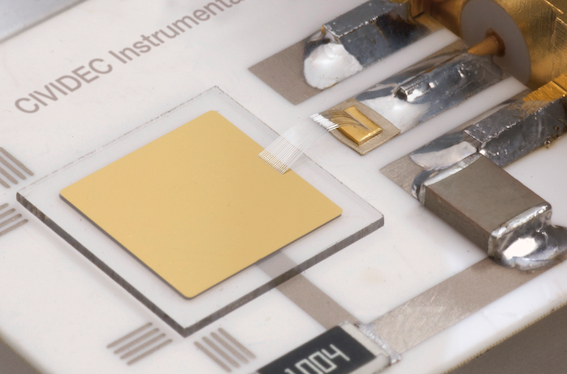
\includegraphics[width=0.7\textwidth]{01_introduction/pics/cividecpcvd}
\caption{A pCVD diamond pad detector \cite{Cividec:00000}.}
\label{fig:cividecpcvd}
\end{figure}

Under a carefully controlled pressure and temperature conditions with an added abrasive atomic hydrogen the graphitic bonds break and form into diamond bonds. The speed of the growth can be anywhere between 0.1 and 10~$\upmu$m per hour. The detector grade samples are grown at a rate of the order of 1~$\upmu$m per hour. They can grow up to several millimetres in thickness. The width of the samples, however, depends entirely on the substrate used. Diamond can be deposited on various materials: diamond, silicon, tungsten, quartz glass etc. The substrate material must be able to withstand the high temperatures during the CVD process. The diamond substrate does not need any surface pre-treatment. Carbon atoms form bonds with atoms in the existing crystal structure. This is the homo-epitaxial growth where the newly deposited atoms retain the orientation of the structure in the substrate. Other non-diamond substrates, however, need to be pre-treated, usually by being polished using diamond powder. Some powder particles remain on the surface, acting as seeds for the growth of small crystals or grains. These grains grow and at some point merge with the adjacent ones, making up a compact material. The lower side is later polished away. These diamonds are called \emph{polycrystalline} (pCVD) whereas those grown on a diamond substrate are \emph{single crystal} (sCVD) diamonds. The area of the former can be large - up to 0.5~m$^2$ or more compact 75~cm$^2$ in the case of detector grade diamonds, which can be further cut into smaller parts. The sCVD diamonds, on the other hand, can currently only achieve sizes up to 1.5~cm$^2$.
\end{description}




%----------------------------------------------------------------------------------------------------
\section{Semiconductor detectors}
Semiconductor is a class of solids whose electrical conductivity is between that of a conductor and that of an insulator -- of the order of  $10^{-5}~\Upomega^{-1}$~cm$^{-1}$. Semiconductors consist of atoms with four electrons in their valence band, e.g. silicon--Si or germanium--Ge, or as combinations of two or more different materials, e.g. gallium arsenide--GaAs). The atoms in the lattice form valence bonds with adjacent atoms, creating solid crystal structures.

Semiconductor particle detectors are devices that use a semiconductor material to detect radiation. They work on the principle of an ionisation chamber. An incident particle ionises the atoms in the crystal lattice. The charges are freed if the deposited energy is higher than the energy band gap, i.e. the energy needed to excite an electron from its steady state to the conductance band. The freed charge carriers start drifting in an externally applied electric field, inducing current on the electrodes. The induced signal is amplified and read out by the electronics in the detector signal chain.

Semiconductor detectors are most widely used for tracking applications, like the Insertable B-Layer shown in figure~\ref{fig:ibl}~\cite{Pernegger:1985432}, which was installed in ATLAS Experiment in 2014. First, they can be produced in thin layers to minimise the impact on the path of the incident particles. Second, their low sensor capacitance allows for a fast signal response. Third, they are highly efficient and highly resistant to radiation damage. Finally, the industrial processes allow for a fine spatial segmentation, which in turn improves the track resolution of the detector systems. 

Semiconductor sensors come in several configurations. The simplest type is a pad -- a single plate with two electrodes. Pads are used for particle counting and radiation monitoring. Next is a strip detector, a more finely segmented detector made out of long parallel sensing areas or strips. Normally each strip has its own signal line for readout. Usually the strip detectors are used in pairs -- one detector is placed on top of the other at an angle to increase spatial resolution in both axes. The third and the most finely segmented is a pixel detector, consisting of a 2D array of independent sensing areas. In tracking applications, pixel detectors are used where the need for a high detection resolution and granularity requirement is the highest. Due to their high production cost and a high number of signal channels, they can only cover limited areas. Strip detectors can be used to cover larger areas in several consecutive layers.

\begin{figure}[!t]
\centering
\includegraphics[width=0.7\textwidth]{01_introduction/pics/ibl}
\caption{The Insertable B-Layer -- a silicon particle tracker installed in the ATLAS experiment in 2014 \cite{MarcelloniDeOliveira:1702006}.}
\label{fig:ibl}
\end{figure}




% ---------------------------------------------------------------------------------------------------------------
%\clearpage
\section{Principles of signal formation in semiconductors}
\label{sec:princsigfor}
% ---------------------------------------------------------------------------------------------------------------
%Lattice, electron-hole pair production (3 pg)
%Ramo theorem (2 pg)
%SC detector systems, pg. 43-73
Particles can interact with the sensor in several ways, e.g. via bremsstrahlung~\cite{BREMS:00000}, elastic or inelastic scattering or nuclear reactions~\cite{PARMA:00000}. Bremsstrahlung is radiation created when a particle is decelerated due to interaction with the electric field of the core of an atom. Elastic scattering is deflection of the particle's trajectory due to the pull from the nucleus without depositing any energy in it. This is in principle an unwanted effect in semiconductors as it deteriorates the spatial resolution of the sensor. Inelastic scattering is the interaction through which an electron in the atom is \emph{ionised}. Nuclear reaction is the direct interaction between the incident particle and the core of the atom. All these effects are competing and are dependent on the particle's mass, momentum etc. The scope of this chapter is to discuss the ionisation mechanism in semiconductors.

The energy of the electrons forming valence bonds between atoms in the crystal lattice is within the \emph{valence band}~\cite{PHSEM:00000}. To break a bond and excite the electron into a \emph{conduction band}, a sufficient energy has to be applied. The minimal energy required is equal to the energy band gap $E_\mathrm{g}$ of the semiconductor. Typical $E_\mathrm{g}$ values are 0.7~eV in Ge, 1.12~eV in Si and 1.4~eV in GaAs. Diamond with its 5.5~eV band gap is considered an insulator. The separation between the conductive and valence band is referred to as \emph{forbidden gap} where no electron states can exist.

An electron excited into the conduction band leaves behind a positively charged ion with a vacancy -- a hole -- in its valence band, as shown in figure~\ref{fig:semilattice9}. A free \emph{electron-hole pair} is thus created. The free electron travels through the crystal until it is recombined with another hole. Similarly the positive charge of the hole attracts a bound electron in the vicinity, causing it to break from the current bond and moving to the vacancy, thus leaving behind a newly created hole. The process continues, making it look like the hole is traveling through the material~\cite{PHSEM:00000}. 

Both the electron and the hole are referred to as \emph{charge carriers}. Without an externally applied electrical field, they propagate in random directions. Therefore on average there is no overall motion of charge carriers in any particular direction over time.

However, if an external electric field is applied to the crystalline structure, the free electrons and holes drift toward the positive and negative potential, respectively, as shown in figure~\ref{fig:simpledrift}. While drifting, the charges couple with the electrodes, inducing current in the circuit, which is explained by the Shockley--Ramo theorem below. Upon reaching the electrodes the charges stop inducing the current. The equivalent electrical circuit is shown in figure~\ref{fig:simpledrifteq}.

\begin{figure}[!t]
\begin{tabular}{cccc}
\subfloat[Valence bonds in the crystalline structure can be broken, creating a free electron-hole pair]{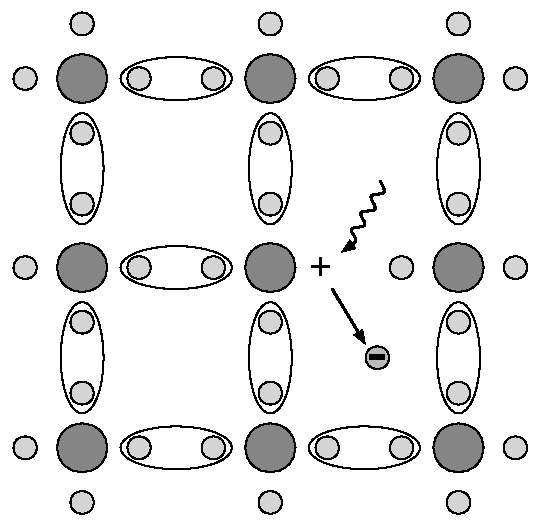
\includegraphics[width=0.22\textwidth]{02_pulse_formation/pics/plots/semilattice9} \label{fig:semilattice9}} &
\subfloat[The freed electron-hole pair starts drifting in the externally applied electric field. The electron and the hole both drift in the opposite directions towards the oppositely charged electrodes.]{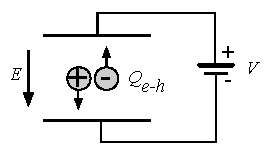
\includegraphics[width=0.32\textwidth]{02_pulse_formation/pics/plots/simpledrift} \label{fig:simpledrift}} &
\subfloat[Equivalent electrical circuit. The moving charges act as a current source.]{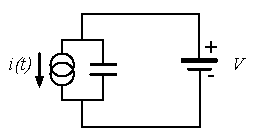
\includegraphics[width=0.34\textwidth]{02_pulse_formation/pics/plots/simpledrifteq}  \label{fig:simpledrifteq}}
\end{tabular}
\caption{In the equivalent electrical circuit diagram the electron-hole creation and drift can be modelled as a current source with a capacitor in parallel.}
\end{figure}





%-----------------------------------------------------------------------------------------------------------------
\subsection{Signal induction by moving charges}
The signal induction in a conducting plane by a point-like charge, which couples with an electrode, is derived in~\cite{PDDC:00000}. The electrode can in this case be modelled as an infinite conducting plane. When a point charge $q$ is created (e.g. an electron-hole pair created via ionisation), its electrostatic field lines immediately couple with the electrode, as seen in figure~\ref{fig:chargeind1}. The electric field on the metal surface due to a point-like charge $q$ at the distance $z_\mathrm{0}$ is
\begin{equation}
E_\mathrm{z}(x,y) = \frac{qz_\mathrm{0}}{2\pi\epsilon_\mathrm{0}(x^2+y^2+z_0^2)^\frac{3}{2}}~~~~~~~~~~E_\mathrm{y} = E_\mathrm{z} = 0.
\end{equation}
\begin{figure}[!t]
%\centering
\begin{tabular}{cccc}
\subfloat[Newly created point charge couples with the conductive plane.]{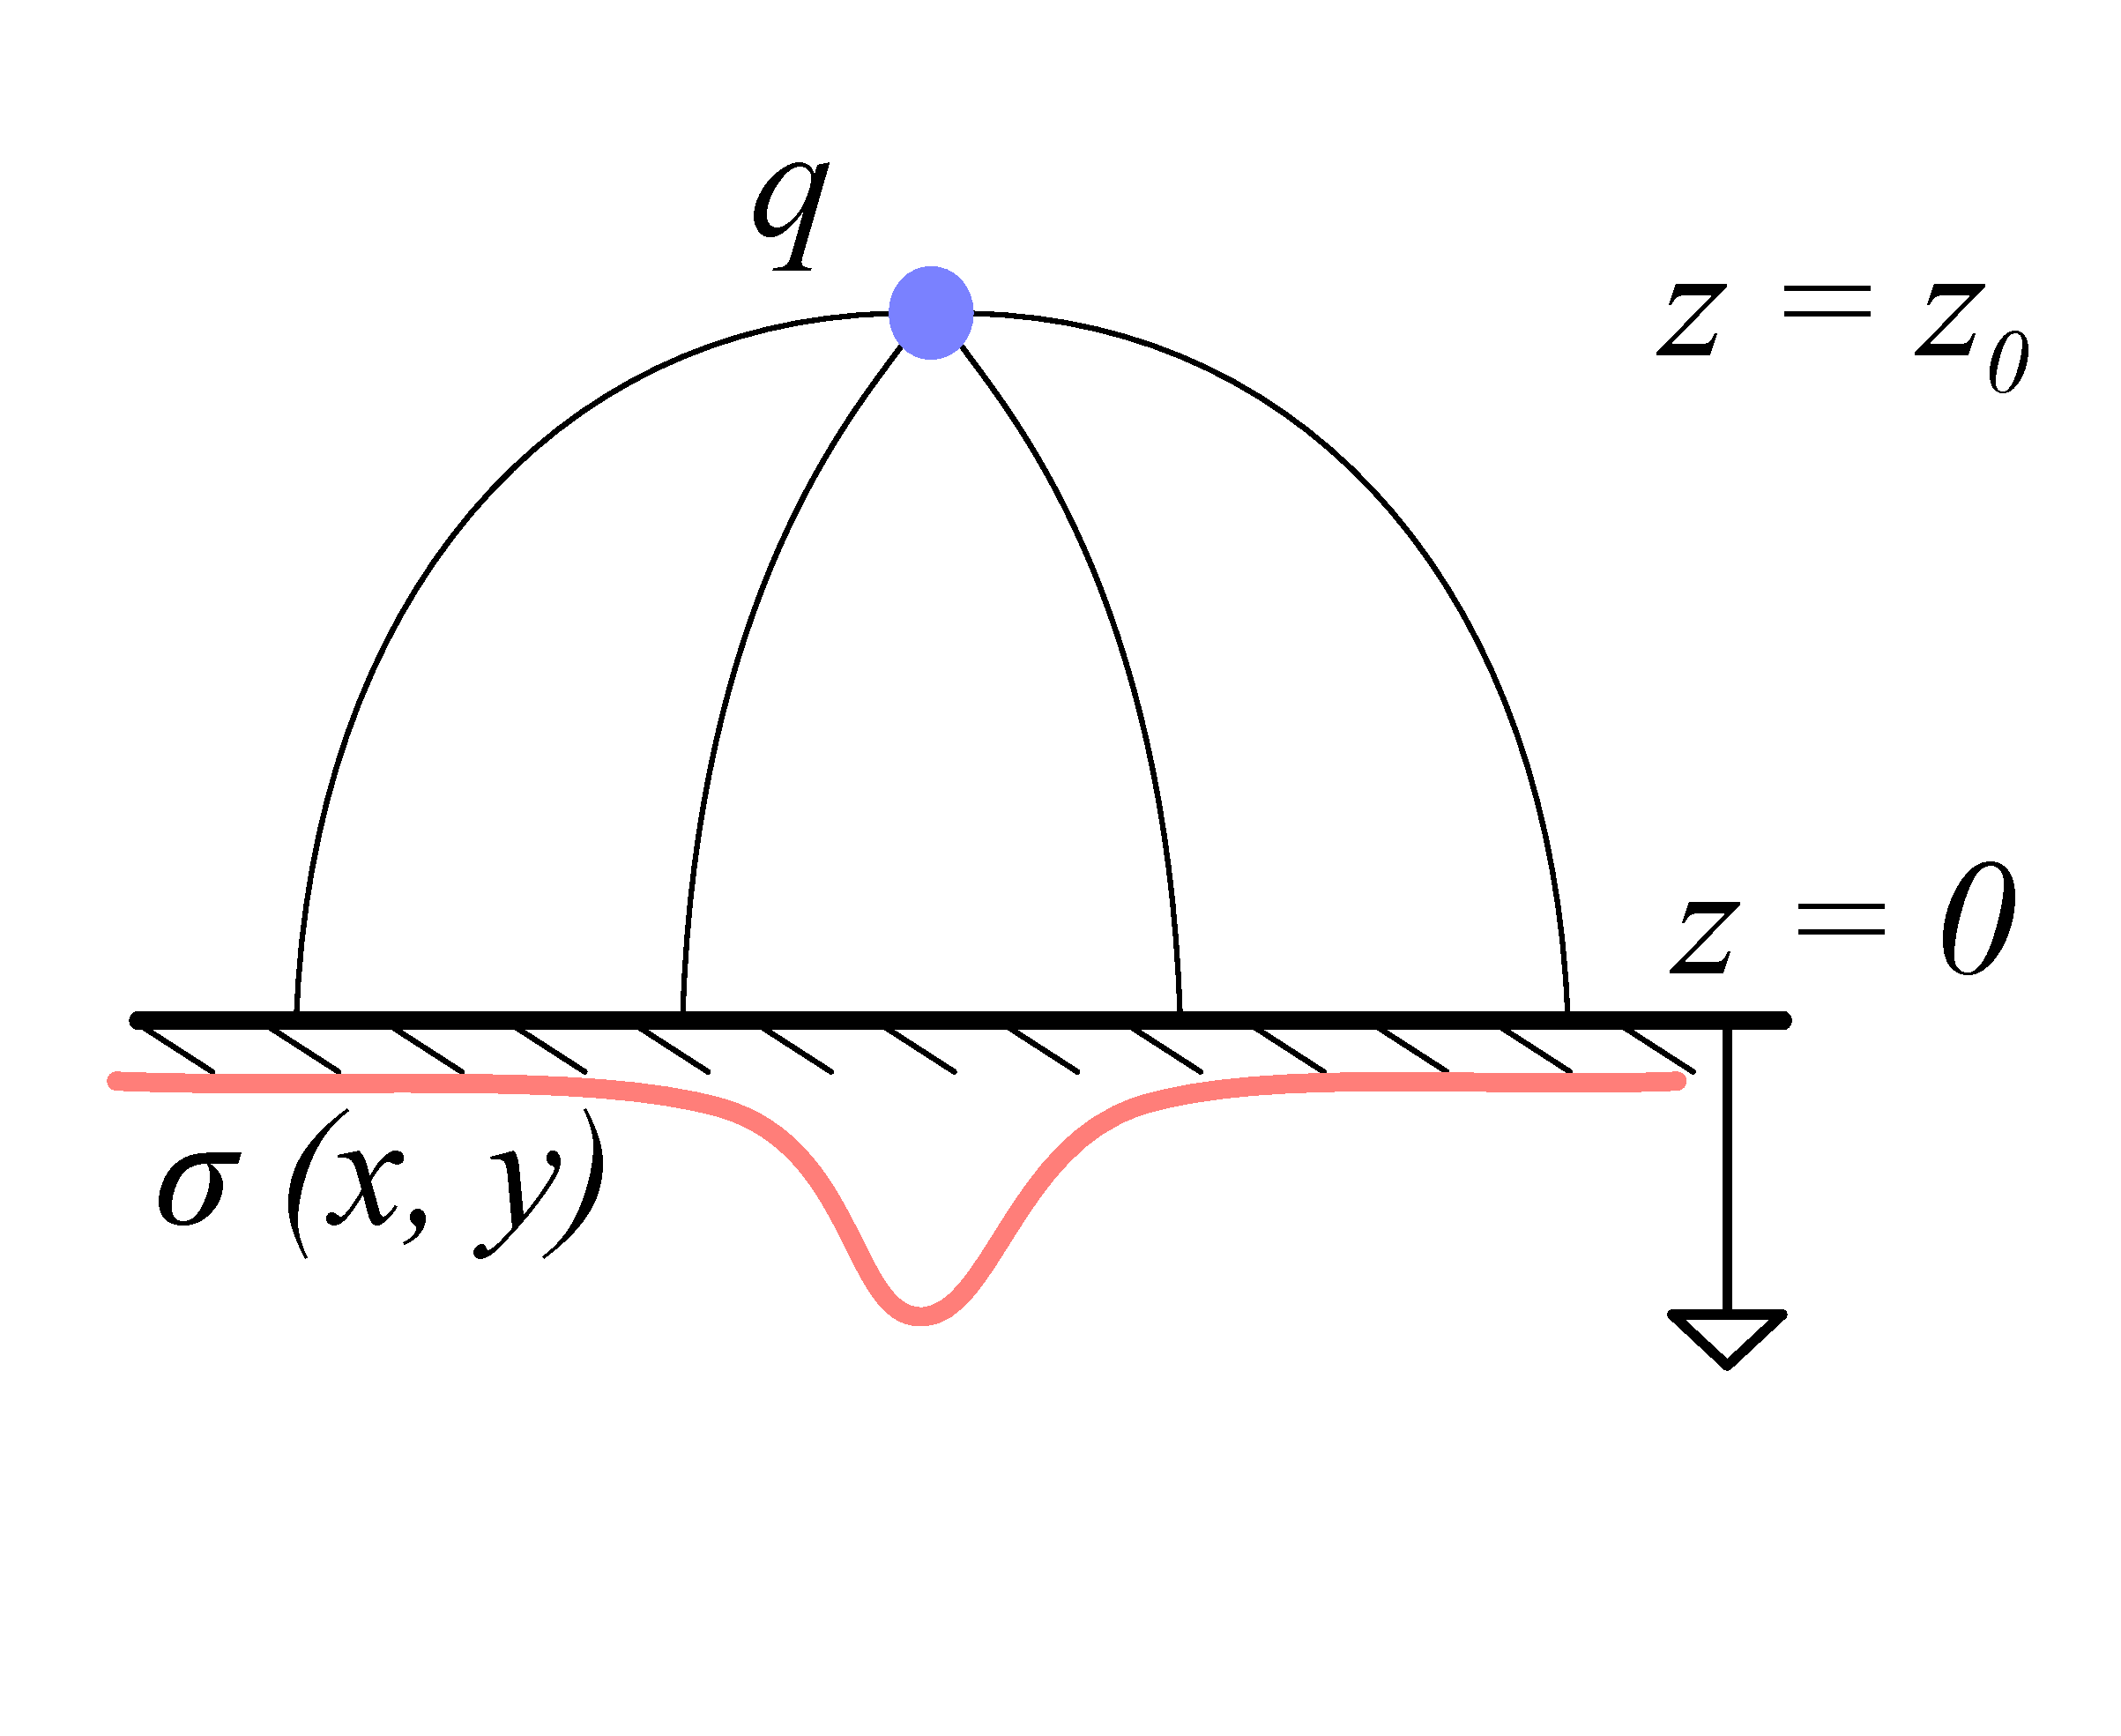
\includegraphics[width=0.30\textwidth]{02_pulse_formation/pics/plots/chargeind1} \label{fig:chargeind1}} &
\subfloat[When the charge drifts, the charge density in the plane changes.]{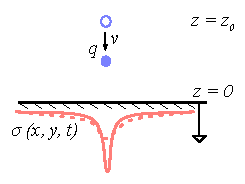
\includegraphics[width=0.30\textwidth]{02_pulse_formation/pics/plots/chargeind2} \label{fig:chargeind2}} &
\subfloat[The changing charge density in the small regions of the plane induces current.]{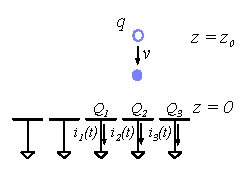
\includegraphics[width=0.30\textwidth]{02_pulse_formation/pics/plots/chargeind3}  \label{fig:chargeind3}}
\end{tabular}
\caption{A point-like charge inducing current in a conductive plane.}
\end{figure}
A mirror charge appears on the conducting plane, with a charge density distribution
\begin{equation}
\label{eq:chgdnstydist}
\sigma(x,y)=\epsilon_\mathrm{0}E_\mathrm{z}(x,y)=\frac{qz_\mathrm{0}}{2\pi(x^2+y^2+z_0^2)^\frac{3}{2}}.
\end{equation}
The charge density integrated over the entire plane yields a mirror charge $Q$, which is an opposite of point charge $q$:
\begin{equation}
\label{eq:chargedensity}
Q=\int_{-\infty}^{\infty} \int_{-\infty}^{\infty} \sigma(x,y)\mathrm{d}x\mathrm{d}y = -q.
\end{equation}
The plane is then segmented into infinitely long strips with a width $w$ whereby each of the strips is grounded, as shown in figure~\ref{fig:chargeind3}. Considering a charge density distribution~\ref{eq:chgdnstydist}, the resulting mirror charge on a single strip $Q_\mathrm{2}$ directly below the point charge $(x=0, y=0)$ yields
\begin{equation}
\label{eq:stripcharge}
Q_\mathrm{2}(z_\mathrm{0})=\int_{-\infty}^{\infty}\int_{-w/2}^{w/2}\sigma(x,y)\mathrm{d}x\mathrm{d}y = -\frac{2q}{\pi}\arctan\left(\frac{w}{2z_\mathrm{0}}\right)
\end{equation} 
If the charge starts moving towards the conducting plane, the mirror charge density distribution also changes, as shown in figure~\ref{fig:chargeind2}. As a result the $Q_2[z(t)]$ changes with time. The changing charge is in effect an induced electric current $i_2(t)$:
 \begin{equation}
 \label{eq:indcurr}
 i_2(t) = -\frac{\mathrm{d}}{\mathrm{d}t}Q_\mathrm{2}[z(t)] = -\frac{\partial Q_\mathrm{2}[z(t)]}{\partial z}\frac{\partial z(t)}{\partial t} = \frac{4qw}{\pi[4z(t)^2 + w^2]}v. 
 \end{equation}
 The movement of the point-like charge therefore induces current in the conducting plane. The induced current is linearly dependent on the velocity of the point-like charge.

%-----------------------------------------------------------------------------------------------------------------
\subsection{Shockley-Ramo theorem}
W. Shockley~\cite{SHOCKLEY:00000} and S. Ramo~\cite{RAMO:00000} independently proposed a theory which explains how a moving point charge induces current in a conductor. The Shockley-Ramo theorem can therefore be used to calculate the instantaneous electric current induced by the charge carrier or a group of charge carriers. It can be used for any number of electrodes. It states that the current $I_\mathrm{n}^{\mathrm{ind}}(t)$ induced on the grounded electrode $n$ by a point charge $q$ moving along a trajectory $\textbf{x}(t)$ reads
\begin{equation}
\label{eq:ramo}
I_\mathrm{n}^{\mathrm{ind}}(t) = -\frac{\mathrm{d}Q_\mathrm{n}(t)}{\mathrm{d}t} =  -\frac{q}{V_\mathrm{w}}\nabla\Psi_\mathrm{n}[\textbf{x}(t)]v(t)  =  -\frac{q}{V_\mathrm{w}}\textbf{E}_\mathrm{n}[\textbf{x}(t)]v(t),
\end{equation}
where $\textbf{E}_\mathrm{n}(\textbf{x})$ is the \emph{weighting field} of electrode $n$ in the case where the charge q is removed, electrode $n$ is  set to voltage $V_\mathrm{w}=1$ and all other electrodes are grounded.  The weighting field is defined as the spatial differential of the \emph{weighting potential}: $\textbf{E}_\mathrm{n}(\textbf{x})=\nabla \Psi_\mathrm{n}(\textbf{x})$. In the case of two parallel electrodes, the weighting field is $E_\mathrm{w} = -\frac{\mathrm{d}\Psi}{\mathrm{d}x} = -1/d$, where $d$ is the distance between the electrodes. The resulting induced current is therefore
\begin{equation}
\label{eq:ramoparallel}
i(t) = \frac{q}{d}v_\mathrm{drift}(x,t),
\end{equation} 
whereby $v_{\mathrm{drift}}$ is the drift velocity of the point-like charge and $d$ is the distance between the electrodes. $d$ is defined by the dimensions of the sensor. The drift velocity is a function of the externally applied electric field, as defined in section~\ref{sec:carrtransp}. If the electric field is set to a constant value, the induced current is directly proportional to the drifting charge. Therefore, by measuring the height of the induced current at a specific point of time the number of moving charges can be deduced.


%moving charge->changed i

%shortened derivation

%i=e/vd


%The energy from an incoming particle can be absorbed by lattice excitation (phonon production) or by ionisation (formation of a mobile charge pair). For a single event, the deposited energy E$_{0}$ is equal to the sum of the energies going into excitation (E$_{ex}$) and ionisation (E$_{ion}$)
%\begin{equation}
%\label{eq:excitationionisation}
%E_0 = E_{ex} N_{ex} + E_{ion} N_{ion}
%\end{equation} 
%where N$_{ex}$ is the number of excitations (phonos produced) and N$_Q$ is the number of charge pairs released. For this event, if more 


%-----------------------------------------------------------------------------------------------------------------
\subsection{Thermal excitation}
Electrons can be thermally excited to the conduction band. The intrinsic concentration of thermally excited electrons $n_\mathrm{i}$ in semiconductors is proportional to\cite{PHSEM:00000}
\begin{equation}
\label{eq:intrinsiccarrier}
n_\mathrm{i} \propto \exp\left(-\frac{E_\mathrm{g}}{2k_\mathrm{B}T}\right)
\end{equation} 
wherein $k_\mathrm{B} = 1.381\times10^{-23}~$m$^2~$kg~s$^{-2}~$K$^{-1}$ is the Boltzmann constant, $E_\mathrm{g}$ is the energy band gap of the semiconductor and $T$ is the temperature in K.
%The thermally excited electrons moving through the material are referred to as leakage current. This current is also present in silicon with an energy gap of 1.12~eV.
Due to the small band gap in semiconductors a significant amount of electrons already occupies the conduction band at room temperature due to thermal excitation, according to the probabilistic distribution. To reduce this effect semiconductor sensors are doped with donors and acceptors, forming a diode~\cite{PHSEM:00000}. The diode is then inversely biased to deplete the material of all free charges. Doped silicon fulfils most of the needs for particle physics requirements and is therefore the most widely used material for particle detection. Diamond with its high energy band gap on the other hand only has a negligible number of thermally excited electrons at room temperature. Therefore a p-n junction is not needed, which simplifies the sensor production.

 

%-----------------------------------------------------------------------------------------------------------------
\subsection{Space charge}
The Poisson equation shows that 
\begin{equation}
\label{eq:poisson}
\frac{d^2\Phi(x)}{\mathrm{d}x^2} = \frac{dE(x)}{\mathrm{d}x} = \frac{\rho(x)}{\epsilon}
\end{equation}
where $\rho(x)$ is the space charge distribution, $E$ is the electrical field and $\Phi$ is the voltage potential. In an ideal diamond, the externally applied high voltage potential on the two electrodes decreases linearly through the sensor. The electrical field is therefore constant throughout the sensor and the space charge distribution across it equals 0. However, space charge may be introduced in the material either by means of accumulating of charge carriers in the lattice (i.e. charge trapping) or already during sensor production. The space charge can be either permanent or changing -- sometimes it is possible to reduce it, as is shown in chapter~\ref{ch:meas}. All in all, it is very important to reduce it because it affects the shape of the electrical signal. Since the drift velocity of the charge carriers is proportional to the electrical field, the charges change their velocity while drifting through the space charge region. Figure~\ref{fig:spcchg} compares the voltage potential, the electrical field and the space charge for an ideal sensor as well as for that with a uniformly distributed positive space charge.
\begin{figure}[!t]
\begin{center}
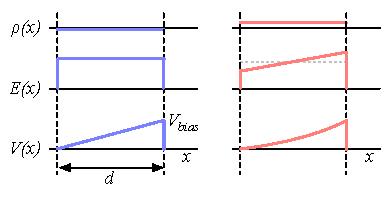
\includegraphics[width=0.6\linewidth]{02_pulse_formation/pics/plots/spcchg}
\caption{Left figure shows a profile of a diamond sensor only with an externally applied electric field. In the figure on the right a uniformly distributed space charge is added in the diamond, contributing to  the internal electric field distribution. The induced current signal is proportional to the electrical field. $d$ is the thickness of the diamond sensor.}
\label{fig:spcchg}
\end{center}
\end{figure}



% ---------------------------------------------------------------------------------------------------------------
%\clearpage
\section{Carrier transport in a diamond sensor} 
\label{sec:carrtransp}
% ---------------------------------------------------------------------------------------------------------------
This section describes the carrier transport phenomena in diamond. This theory provides the basis for discussion about the measurements in chapter~\ref{ch:meas}. 
Table~\ref{tab:semicompare} compares the properties of diamond and silicon. Some of these values are revisited and used in the course of this thesis. 

\begin{footnotesize}
\begin{center}
\begin{tabular}{   l  c  c   }
\hline
Property & Diamond & Silicon \\
\hline
Band gap energy E$_\mathrm{g}$ (eV) & 5.5 & 1.12  \\
Electron mobility $\upmu_\mathrm{e}$ (cm$^2$ V$^{-1}$ s$^{-1}$) & 1800~\cite{Jansen:1956431} & 1500~\cite{PHSEM:00000} \\
Hole mobility $\upmu_\mathrm{h}$ (cm$^2$ V$^{-1}$ s$^{-1}$) & 2500~\cite{Jansen:1956431} & 450~\cite{PHSEM:00000} \\
Breakdown field (V cm$^{-1}$) & $10^{7}$ & $3\times 10^5$ \\
Resistivity ($\Upomega$ cm) & $>10^{11}$  & $2.3\times 10^5$  \\
Intrinsic carrier density (cm$^{-1}$) & $<10^3$ & $1.5\times 10^{10} $ \\
Mass density (g cm$^{-1}$) & $ 3.52$ & $2.33 $ \\
Atomic charge  & $6 $ & $ 14$ \\
Dielectric constant $\upvarepsilon$ & $5.7 $ & $11.9 $ \\
Displacement energy (eV/atom) & $43 $ & $13-20 $ \\
Energy to create an e-h pair  (eV) & $13 $ & $ 3.6$ \\
Radiation length (cm) & $ 12.2$ & $9.6 $ \\
Avg. signal created/$\upmu$m (e) & 36 & 89 \\\hline
\end{tabular}
\captionof{table}{Comparison diamond -- silicon~\cite{PHSEM:00000,Jansen:1956431}.}
\label{tab:semicompare}
\end{center}
\end{footnotesize}
 

When the charge carriers are freed in a semiconductor with no concentration gradient and without an externally applied electric field, they scatter in random directions with a thermal velocity $v_{\mathrm{th}}$~\cite{PHSEM:00000}. Their integral movement due to thermal excitation equals zero. 

\begin{description}

\item[Diffusion] is caused by the concentration gradient. In its presence the integral movement is in the direction of the lower concentration until an equilibrium is reached.
The concentration profile dissolves with time forming a Gaussian distribution with variance $\sigma(t)=\sqrt{Dt}$~\cite{PHSEM:00000} .

\item[Drift] is caused by an externally applied electrical field. In that case the carriers move along the field lines. In a sensor with a high applied field the diffusion contribution is negligible. 

\item[Drift velocity] $v_\mathrm{drift}(E)$ is the speed at which the charge carriers drift through the diamond sensor~\cite{PHSEM:00000}.

\item[Mobility] $\mu$ is a proportionality factor between the $v_\mathrm{drift}$ and the electric field $E$ at low electric fields: $v_\mathrm{drift} = \mu E$. Its units are in cm$^2$V$^{-1}$s$^{-1}$.

\item[Phonon transport] is the transfer of energy of the moving charges to the lattice.

\item[Saturation velocity] $v^e_\mathrm{sat}$ is a velocity limit above which the carriers cannot reach. This is due to increasing phonon transport at a high electric field. The $v^e_\mathrm{sat}=v^h_\mathrm{sat}=(14.23\pm0.12)\times10^6$~cm/s for both positive and negative charge carriers has been derived from the measurements in~\cite{JANSEN:00001}.

\end{description}

 The final equation for $v_\mathrm{drift}$ is therefore~\cite{VDRIFT:00000}
\begin{equation}
\label{eq:vsat}
v_\mathrm{drift}(E) = \mu(E)E= \frac{\mu_\mathrm{0} E}{1 + \frac{\mu_\mathrm{o} E}{v_\mathrm{sat}}}.
\end{equation}
It can be retrieved experimentally via the transit time measured with the Transient Current Technique (TCT). This technique enables the measurement of transit time $t_\mathrm{t}$ of the carriers through the sensor with the thickness $d$. 
\begin{equation}
\label{eq:vsat}
v_\mathrm{drift}(E) = \frac{d}{t_\mathrm{t}(E)}.
\end{equation}
The velocities for holes and electrons usually differ. In diamond, the holes travel approximately 30~\% faster than electrons at the room temperature~\cite{Jansen:1956431}.


%-----------------------------------------------------------------------------------------------------------------
\section{Radiation-induced current signals}

\begin{figure}[!t]
\begin{center}
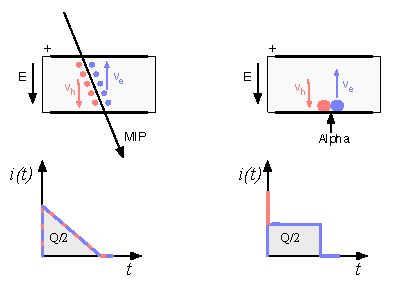
\includegraphics[width=0.7\linewidth]{02_pulse_formation/pics/plots/driftboth}
\caption{Charge carrier drift in diamond for $\upbeta$ and for $\upalpha$ particles crossing the sensor at $t=0$.}
\label{fig:drift}
\end{center}
\end{figure}

When a highly-energetic particle travels through the sensor, it interacts with atoms in the lattice. It ionises the valence electrons, creating electron-hole (e-h) pairs on its way. It can either deposit only a fraction of its energy and exit the sensor on the other side or it can get stopped in the sensor, depositing all of its energy. A special case is when it interacts with the core of the atom in the middle of the sensor by means of a a nuclear interaction. All these various types interactions produce different amounts and different spatial distributions of e-h pairs. 

%The induced electrical current therefore differs for different types of interaction. 
The two most frequent types are shown in figure~\ref{fig:drift}. The first figure shows the interaction of an incident MIP. The electrons and holes created all along the trajectory of the particle immediately start drifting towards the positive and negative electrode, respectively. At $t=0$ all charges drift, contributing to the maximum induced current. Those closest to the electrodes have a very short drift path. They stop inducing current upon reaching the electrode. The resulting current signal is a triangular pulse with a sharp rising edge and a linear falling edge. Gradually all the charge carriers reach the electrode. The accumulated charge $Q_\mathrm{s}$ equals to the sum of the contributions of the positive and negative charge carriers. 

The second type of interaction happens when the particle is stopped in the diamond close to the point of entry. Most of its energy is deposited in a small volume close to the electrode. A cloud of charge carriers is created and the charges with the shorter path to the electrode disappear almost instantly. The carriers of the opposite charge, however, start drifting through the sensor to the other electrode. In an ideal diamond sensor, their velocity is constant throughout the drift up until they are collected at the opposite electrode. The contribution of the first charge cloud is a peak with a short time. The cloud drifting through the sensor, on the other hand, induces a current signal with a flat top. The resulting signal has a shape of a rectangle, with a spike in the beginning. %This spike is filtered out by a current amplifier in a real device because it is too fast for the electronics existing currently. 
The accumulated charge $Q_\mathrm{s}$ is equal to a half of the deposited charge by the stopped particle.

The two aforementioned types of interactions have well defined signal responses. Nuclear interactions on the other hand yield various results. The resulting signal shape depends on the decay products of the interaction, which can be $\upalpha$, $\upbeta$ or $\upgamma$ quanta or other nuclei, inducing a mixed shaped signal. 

%----ADD!!!!!!!!!-----------\
%\subsection{Transient Current Technique}
%The Transient Current Technique (TCT)

%-----------------------------------------------------------------------------------------------------------------
\subsection{Mean energy loss}
A mean energy loss of a particle traversing the detector as a function of the momentum is given with the Bethe-Bloch equation~\cite{BETHE:00001}: 
\begin{equation}
-\left\langle\frac{\mathrm{d}E}{\mathrm{d}x}\right\rangle = \frac{4\pi}{m_\mathrm{e}c^2}  \cdot \frac{nz^2}{\beta^2}  \cdot  \left(\frac{e^2}{4\pi\epsilon_\mathrm{0}}\right)^2  \cdot  \left( \ln \left(\frac{2m_\mathrm{e}c^2\beta^2}{I\cdot(1-\beta^2)}\right)-\beta^2  \right)
\label{eq:bethebloch}
\end{equation}
The resulting function for a muon is shown in figure~\ref{fig:bb2}. At a momentum of around 300~MeV/c the incident particle deposits the lowest amount of energy. Hence it is referred to as the \emph{minimum ionising particle} or a MIP.


\begin{figure}[!t]
\begin{center}
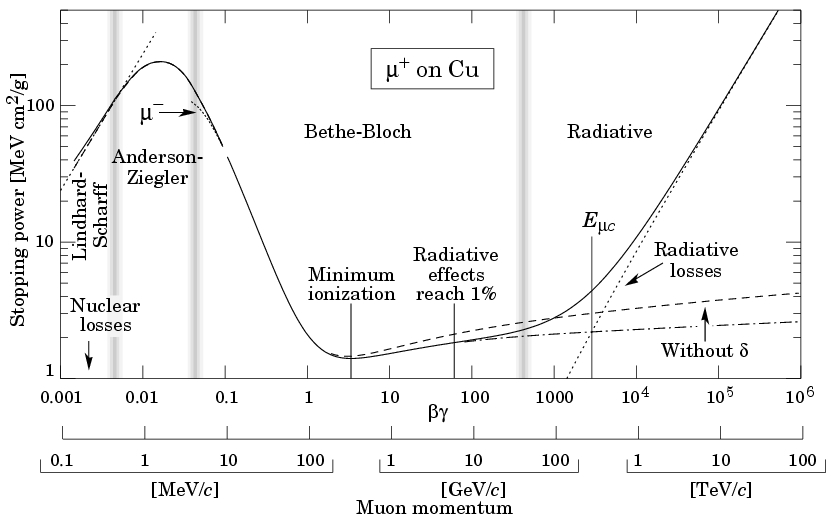
\includegraphics[width=0.7\linewidth]{02_pulse_formation/pics/bb2}
\caption{Stopping power for muons according to the Bethe-Bloch formula~\cite{BETHE:00001}.}
\label{fig:bb2}
\end{center}
\end{figure}

%-----------------------------------------------------------------------------------------------------------------
\subsection{Signal fluctuation}
Two important sensor properties are the magnitude of the signal and the fluctuations of the signal at a given absorbed energy. They determine the relative resolution $\Updelta E/E$. For semiconductors the signal fluctuations are smaller than the simple statistical standard deviation $\upsigma_\mathrm{Q}=\sqrt{N_\mathrm{Q}}$. Here $N_\mathrm{Q}$ is the number of released charge pairs, i.e. the ratio between the total deposited energy $E_\mathrm{0}$ and the average energy deposition $E_\mathrm{i}$ required to produce an electron-hole pair. \cite{1947PhRv...72...26F} shows that the standard deviation is $\upsigma_\mathrm{Q}=\sqrt{F N_\mathrm{Q}}$, where $F$ is the Fano factor~\cite{1947PhRv...72...26F} (0.08 for diamond and 0.115 for silicon ~\cite{1980PhRvB..22.5565A}). Thus, the standard deviation of the signal charge is smaller than expected, $\upsigma_\mathrm{Q}\approx0.3 \sqrt{N_\mathrm{Q}}$. The resulting intrinsic resolution of semiconductor detectors is 
\begin{equation}
\label{eq:efwhm}
\Updelta E_\mathrm{FWHM} = 2.35 \sqrt{FEE_\mathrm{i}} 
\end{equation} 
wherein $E_\mathrm{i}(Si)$=~3.6~eV and E$_\mathrm{i}(Di)$=~13~eV. E.g., for an $\upalpha$ particle with energy $E_\upalpha$ = 5.5 MeV the calculated resolution in diamond is equal to $\Updelta E_{\mathrm{FWHM}}$ = 5.6~keV. This defines the minimum achievable resolution for energy spectroscopy with semiconductors. 
%Figure~\ref{fig:enerres} shows the resolution limit as a function of energy in silicon and diamond.
%
%\begin{figure}[!t]
%\begin{center}
%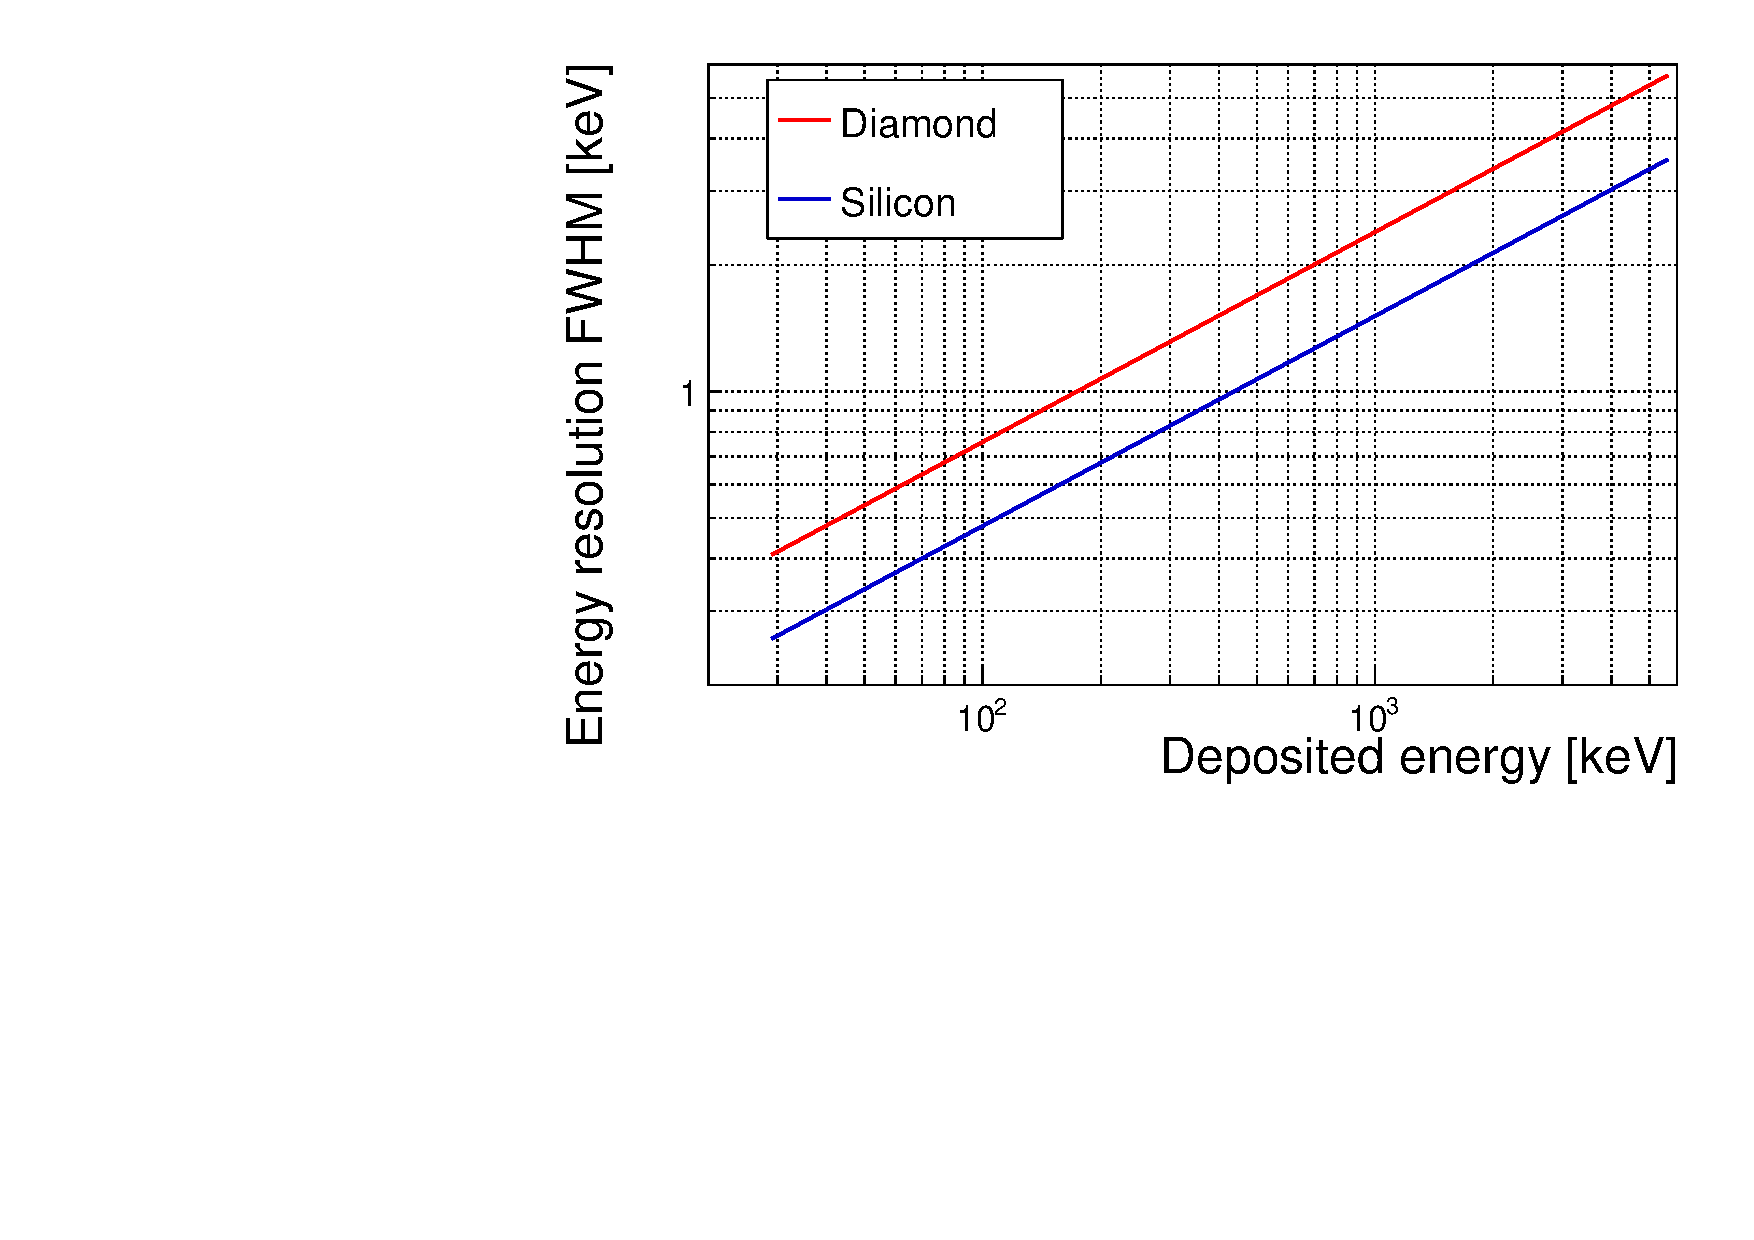
\includegraphics[width=0.7\linewidth]{../scripts/02_pulse_formation/plots/resolution}
%\caption{Calculated intrinsic energy resolution for silicon and diamond.}
%\label{fig:enerres}
%\end{center}
%\end{figure}


%-----------------------------------------------------------------------------------------------------------------
\subsection{Charge collection}
The total measured charge $Q_\mathrm{i}$ is the integral of the induced current:
\begin{equation}
Q_\mathrm{i}=\int i_\mathrm{ind}(t) \mathrm{d}t.
\end{equation}
The expected charge $Q_\mathrm{0}$ can be calculated using the thickness of the sensor $d$ and the average number of e-h pairs created per $\upmu$m $\delta_\mathrm{d}$, which is 36~e-h/$\upmu$m for diamond according to table~\ref{tab:semicompare}. 
The expected charge created by a MIP flying through a sensor with a thickness $d=500~\upmu$m perpendicular to the electrodes is
\begin{equation}
\label{eq:qBeta}
Q_\mathrm{MIP}=\delta_\mathrm{d}\cdot d \cdot q = 18\times10^3~\mathrm{eh} \cdot q = 2.9~\mathrm{fC}
\end{equation}
where $q=1.6\times10^{-19}$~C is the elementary charge.
If a particle stops in the sensor, it deposits all its energy. In this case the number of created e-h pairs is calculated according to equation~\ref{eq:qAlpha} using $E_\mathrm{eh}$, the energy required to create an e-h pair. For diamond this value is 13, according to table~\ref{tab:semicompare}. For a 5.5~MeV $\upalpha$ particle emitted from an $^{241}Am$ source the expected charge is
\begin{equation}
\label{eq:qAlpha}
Q_\upalpha = \frac{E}{E_\mathrm{e-h}} \cdot q = \frac{5.5~\mathrm{MeV}}{13~\mathrm{eV}} \cdot q = 4.25\times10^5~\mathrm{eh} \cdot q = 68~\mathrm{fC}.
\end{equation}
where $E$ is the energy of the incident particle.
which is almost for a factor of 24 larger than expected charge of a MIP. The charge collection efficiency (CCE) is the ratio between the measured and expected charge:
\begin{equation}
\label{eq:ccecalc1}
CCE = \frac{Q_\mathrm{i}}{Q_\mathrm{0}} = \frac{Q_\mathrm{i}}{\delta_\mathrm{d}\cdot d}\cdot100\%.
\end{equation}
The charge collection distance (CCD) is a measure of an average path that the charge carriers travel before getting trapped:
\begin{equation}
\label{eq:ccdcalc1}
CCD = \frac{Q_\mathrm{i}}{\delta_\mathrm{d}}
\end{equation}
and is usually given in units of $\upmu$m.

Carriers that get trapped stop contributing to the overall induced current on the electrodes. The more charges are trapped along their drift path, the more the current induced on the electrodes is decreased. This in turn yields a lower integrated charge. 
An expected CCE for non-irradiated sCVD diamonds is close to 100~\%. For highest quality non-irradiated pCVD diamonds it ranges between 40~\% and 60~\%. In other words, high-quality pCVD diamonds already have traps introduced by means of grain boundaries, which are created in the growing process. Traps can also be created by damaging the diamond using radiation (discussed in section~\ref{sec:raddam}). The more the sensor is irradiated, the larger number of traps is introduced in the material and the higher is the probability that the carriers are stopped on the way, reducing in turn the integrated charge. Therefore the CCD and CCE can be used as a means to quantify the detector damage due to radiation.

%-----------------------------------------------------------------------------------------------------------------
\subsection{Charge trapping}
Various types of lattice defects can be created in diamond, similar to those in silicon~\cite{CHTR:00000}.
Figure~\ref{fig:raddamage} shows several examples of lattice damage:
\begin{enumerate}
\item[a)]foreign interstitial (e.g. H, Li),
\item[b, c)]foreign substitutional (e.g. N, P, B),
\item[d)]vacancy and
\item[e)]self interstitial.
\end{enumerate}
\begin{figure}[!t]
\begin{center}
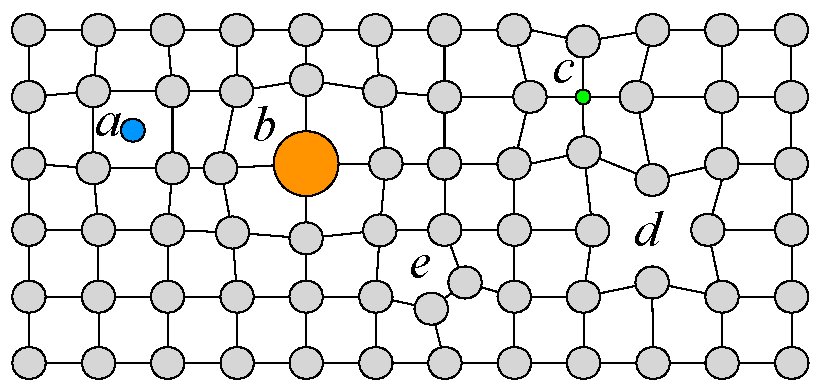
\includegraphics[width=0.55\linewidth]{02_pulse_formation/pics/plots/raddamage}
\caption{Impurities and non-uniformities in the crystal lattice due to radiation damage.}
\label{fig:raddamage}
\end{center}
\end{figure} 
These non-uniformities form new energy levels in the forbidden gap. These intermediate levels are referred to as charge traps because they can trap moving charge carriers. The energy level of the trapped carriers is reduced from the conduction band to the energy level of the trap. Different types of lattice damage have different energy levels. The carriers trapped in a shallow trap -- an energy level close to the conduction band -- have a high probability of being thermally excited back into the conduction band whereby they continue drifting towards the electrode. Their activation energy is therefore low. Those trapped in a deep trap close to the middle of the forbidden gap need a much higher activation energy, which in turn increases the average time to their release due to thermal excitation.

The energy band jumping goes the other way, too. The carriers in the valence band may use the intermediate energy levels as ``stepping stones'' to jump to the conduction band and start drifting in the externally applied electric field. These intermediate energy levels are referred to as the generation centres of leakage current.

The charge carriers that drift through the bulk get stopped in the charge traps with a certain probability. This trapping happens uniformly throughout the diamond. In other words, the number of carriers in the moving charge cloud is gradually reduced. This in turn reduces the induced current. The number of drifting carriers per unit of length follows a decaying exponential function
\begin{equation}
\label{eq:decayexp}
I(t)= I_0 + I(0) \cdot e^{-\frac{t-t_0}{\tau} },
\end{equation}
where $I(0)$ is the initial induced current, $I_0$ is the end current, $t$ is time, $t_0$ is temporal displacement of the pulse and $\tau$ is the decay time constant. This value describes how long it takes before the amplitude of the pulse decreases to 63~\% of its initial height.

\subsubsection{Priming/pumping}
Priming or pumping~\cite{pumping:00000} is a process of irradiating the diamond with ionising radiation with a goal to improve the sensor properties. The pumping process strongly reduces the concentration of active carrier trapping centres. This leads to an enhancement of electronic properties of such material. The improved transport properties due to a reduced number of active charge traps give rise to an increased charge collection efficiency. The diamond is usually pumped for a few hours using a strong $\upbeta$ source, preferably a $^{90}Sr$ source with the activity of at least 50~MBq. The diamond remains in a pumped state from a few minutes to several days, depending on the quality of the material. A direct exposure to light results in an immediate return to an non-pumped state.



%-----------------------------------------------------------------------------------------------------------------
\section{Radiation damage}
\label{sec:raddam}
Exposure to ionising radiation degrades sensors by deforming the crystal lattice and introducing charge traps in the material. 

Radiation damage varies with the type of radiation and its energy. There are several models existing~\cite{2002NIMPA,Guthoff:2014223} that try to explain the impact of irradiation and to provide \emph{damage factors} to compare the radiation damage between different particles. The standard way is to convert the damage into \emph{1~MeV neutron equivalent fluence}~\cite{NEQ:00000}. Some models have been extensively verified with simulations and with experiments. In these experiments the charge collection in sensors is measured before and after irradiation. This procedure is repeated several times, with a measurement point taken after every irradiation. Then the charge collection for this set of measurements is plotted as a function of the radiation dose received by a specific particle at a specific energy. From this a damage factor $k_\mathrm{\lambda}$ can be extracted. Damage factors have to be measured across a range of energies and types of radiation to properly quantify the damage in the sensors. Finally they are compared to the simulations to validate the theoretical models.

Diamond is an expensive material and the technology is relatively new as compared to silicon. Therefore few institutes are carrying out diamond irradiation studies. To join the efforts, the RD42 collaboration~\cite{RD42:00000} has been formed. It gathers the experimental data from diamond irradiation studies. Unlike with silicon, the experimental results so far show no significant correlation with the NIEL (non-ionising energy loss) model~\cite{2002NIMPA}, which correlates detector efficiency with the number of lattice displacements. Therefore an alternative model was proposed~\cite{Guthoff:2014223}, correlating the diamond efficiency with the number of displacements per atom (DPA) in the material. The idea is that if the recoil energy of an incident particle is higher than the lattice binding energy (42~eV for diamond), the atom is displaced from its original position. The newly formed vacancy acts as a trap for drifting charge carriers. The more displacements that form in the crystal, the higher is the probability that a drifting carrier gets trapped. However, different types of particles interact differently with the material. In addition the mechanisms of interaction at low energies are different to those at high energies. To assess the damage for individual particles at a range of energies, simulations need to be run first. The simulation shown in~\cite{Guthoff:2014223} shows the DPA model for a range of energies of proton, pion and neutron irradiation in diamond. Figure~\ref{fig:kitdpa}  contains the simulation results as well as the superimposed empirical results of several irradiation studies. According to the figure, a 300~MeV pion beam damages the diamond material twice as much as a 24~GeV proton beam. The data points obtained by RD42 are also added to the figure. They have been normalised to damage by 24~GeV protons. This value has been chosen because radiation damage at this energy and radiation type is well understood at CERN.
%Finally, the data point measured in the scope of this thesis has been added for comparison. The derivation is done below. $ADD SOMEWHERE ELSE!!

\begin{figure}[!t]
\begin{center}
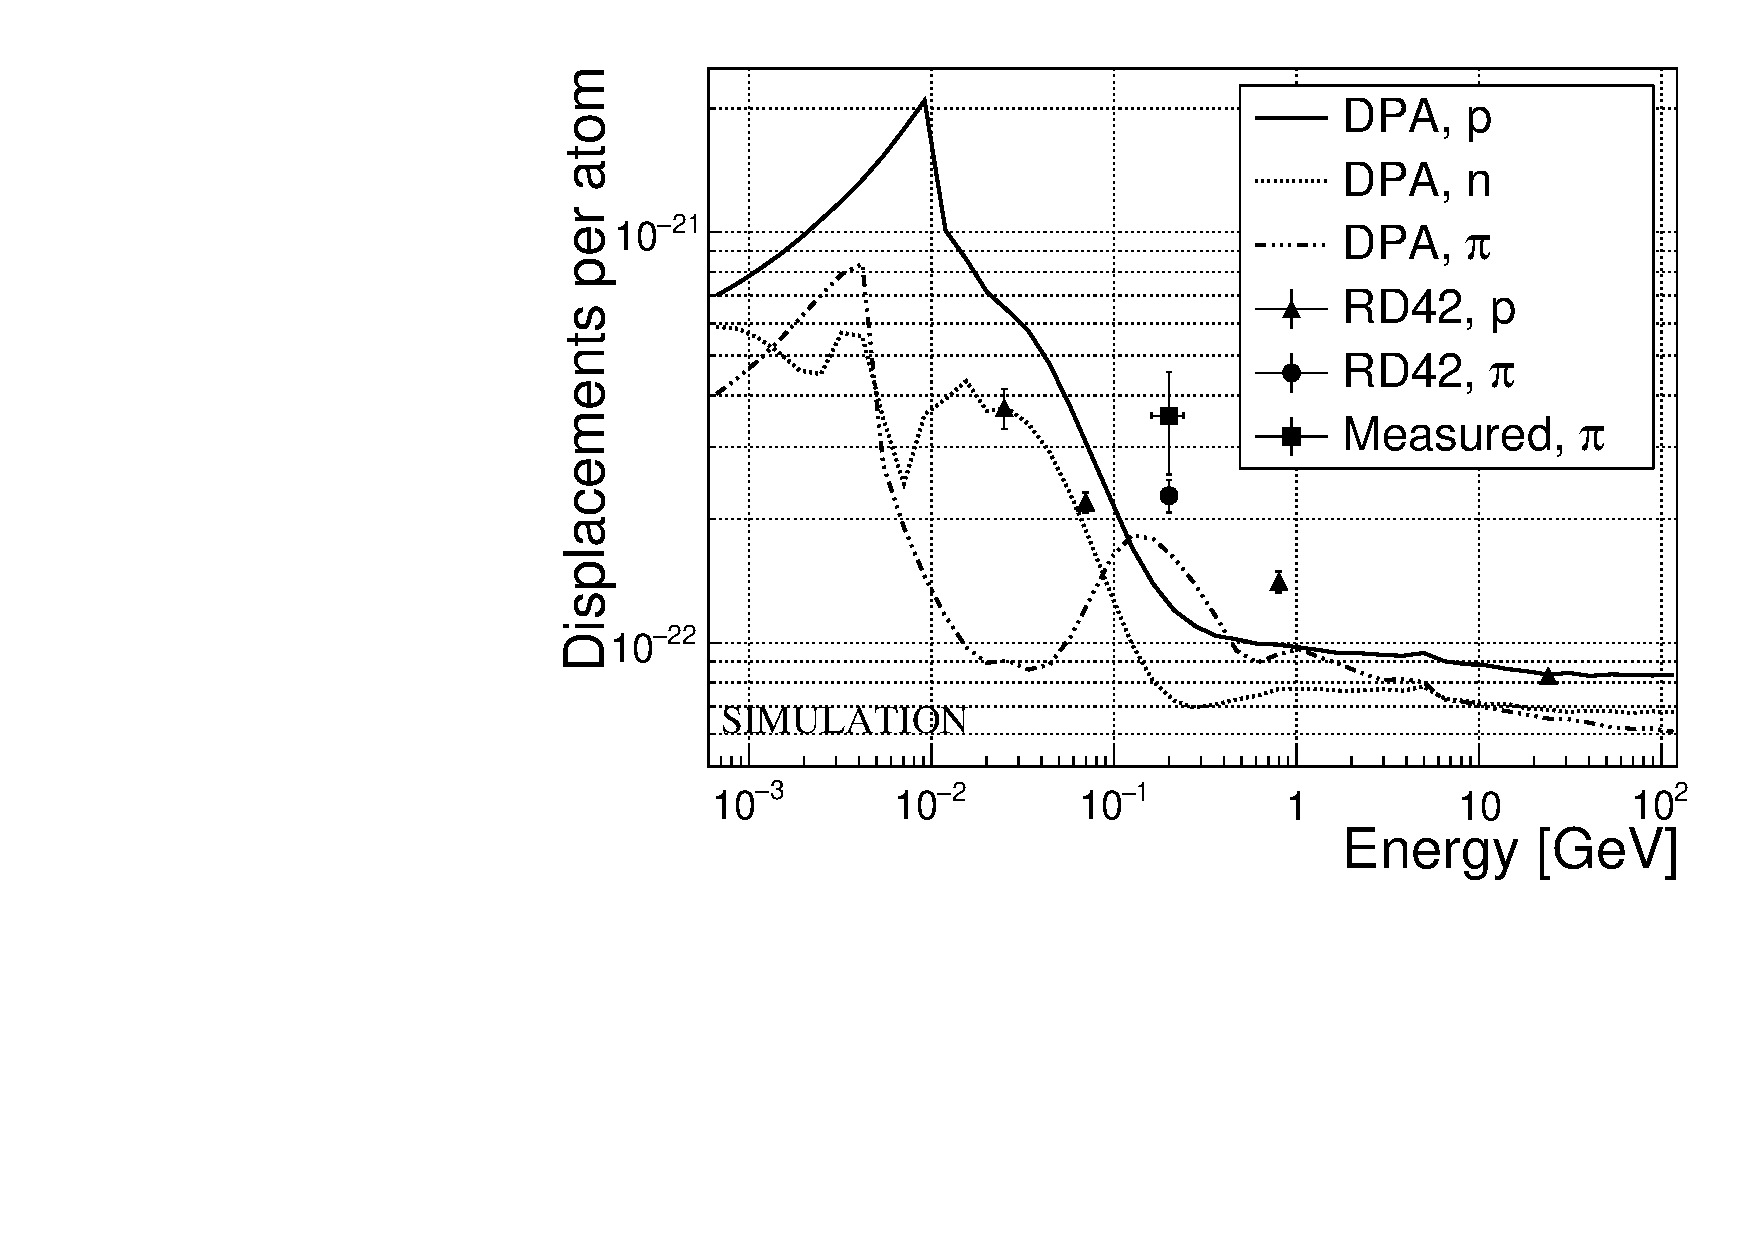
\includegraphics[width=0.7\textwidth]{03_measurement_results/scripts/plots/dpa1}
\caption{Diamond radiation damage - a model based on displacements per atom~\cite{Guthoff:2014223}. The figure shows the DPA as a function of the kinetic energy for protons, neutrons and pions. Added are data points for protons and pions by RD42~\cite{RD42IRRAD:00000}. %and one data point for pions measured in the scope of this study.
}
\label{fig:kitdpa}
\end{center}
\end{figure}

%-----------------------------------------------------------------------------------------------------------------
\subsubsection{Irradiation damage factor}
The irradiation damage factor $k_\uplambda$ is a means to quantify irradiation damage of a specific type of radiation at a specific energy. Via this factor different types of irradiation can be compared. It is obtained experimentally by measuring the CCD of a number of samples at various irradiation steps and fitting the equation~\ref{eq:radfactor1} to the data. $\lambda$ is the measured CCD, $\lambda_\mathrm{0}$ is the CCD of a non-irradiated sample and $\Phi$ the radiation dose. As a reference, the damage factor for 24~GeV protons is set to $1\times10^{-18}~\upmu$m$^{-1}$~cm~$^{-2}$.


\begin{equation}
\label{eq:radfactor1}
\frac{1}{\lambda} = \frac{1}{\lambda_\mathrm{0}}+k_\uplambda\cdot\Phi
\end{equation} 
%\begin{equation}
%\label{eq:radfactor1}
%\lambda = \frac{\lambda_\mathrm{0}}{k_\uplambda \lambda_0 \Phi + 1}
%\end{equation} 





%-----------------------------------------------------------------------------------------------------------------
\section{Temperature effects}
The band gap energy in diamond is equal to $E_\mathrm{g}=5.5$~eV while the average energy to produce an electron-hole pair is $E_{\mathrm{e-h}}=13$~eV. This means there is excessive energy deposited in the diamond bulk. An incident $\upalpha$-particle stops within $\sim$10--15~$\upmu$m of the bulk, transferring all its energy to the lattice during deceleration. A part of this energy directly ionises the carbon atoms, creating free electron-hole pairs. 

The remaining energy, however, is converted into lattice vibrations -- phonons~\cite{PhysRevLett.13.13, Jansen:1956431}. In other words, the lattice within the ionisation volume  of approximately $\sim$15~$\upmu$m $\times\sim$2~nm~\cite{Jansen:1956431} is briefly heated up. The hot plasma then cools down to the temperature of the surrounding material by means of heat dissipation, i.e. phonon transport.

The free electron binds with the free hole into a bound state (not recombination) -- the exciton~\cite{1970PhyEd...5..226L}. The exciton binding energy is 80~meV, which introduces an energy level within the forbidden gap just under the conduction band. At higher temperatures the lattice provides enough energy to thermally excite the electron from the exciton state back to the conduction band. At lower temperatures, however, the exciton lifetime increases, which means that it takes a longer time for the electrons to get re-excited to the conduction band. The re-excitation lifetime at room temperature is $\sim$30~ps, increasing to $\sim$150~$\upmu$s at 50~K~\cite{Jansen:1956431}. This means that some of the bound electrons do not even start drifting within the period of $\sim$10~ns, which is the expected carrier drift time. When they are finally freed, the current they induce is already hidden in the electronics noise. The effective area of the observed current pulse is therefore smaller than that of a pulse induced by all the carriers drifting at the same time. This in effect reduces the measured collected charge. The longer the time constant, the lower the measured collected charge, as shown in section~\ref{subsec:qvst}.

\subsubsection{Collected charge as a function of temperature}
\label{subsec:qvst}
The area below the current pulse is proportional to the charge collected by the diamond detector. The collected charge is measured as a function of temperature. First, the amplitude values of the averaged pulses at a bias voltage of $\pm$500~V and across the temperature range between 4~K and 295~K have to be integrated. Then a calibration factor is used to derive the charge for all data points. The results of such measurements have been presented in~\cite{Jansen:1956431}. Chapter~\ref{ch:meas} shows the results of the measurements taken in the scope of this thesis.
%The resulting values for electrons and holes are plotted in figures~\ref{fig:chgtempelecs} and~\ref{fig:chgtempholes}, respectively.
%ADD!!!!!!!!!!!!!!!!!!!!!!!!!!!!!!!!!!!!!!!!!!!!







% ---------------------------------------------------------------------------------------------------------------
%\clearpage
\section{Electronics for signal processing} % signal acquisition
% ---------------------------------------------------------------------------------------------------------------
\label{sec:elecsigproc}
This section describes the electronics of a detector, starting with a description of signal amplifiers and then discussing the digitisation and signal processing. All these stages are necessary to extract information from the sensor. First, the signal has to be amplified. Then it is digitised and finally processed in a specially designed processor or a logic unit.

\subsection{Signal preamplifiers}
The signal charge generated in the sensor by a single energetic particle is of the order of a few fC. The range of the induced current for single particles is typically between $10^{-8}$~A ($\upbeta, \upgamma$ radiation) and $3\times10^{-7}$~A ($\upalpha$ radiation). Signals as low as these have to be pre-amplified before processing. Depending on the measurement, several types of signal amplifiers can be used. The preamplifiers are designed to minimise electronic noise while maximising gain, thus maximising the signal-to-noise ratio (SNR). In addition, a bandwidth limit must be optimised to minimise the information loss due to signal shape deformation. A critical parameter is the total capacitance, i.e. the sensor capacitance together with the capacitance load of the preamplifier. The SNR improves with a lower capacitance. Several types of amplifiers can be used, all of which affect the measured pulse shape. Two preamplifiers are used most commonly, a current and a charge sensitive amplifier. Both are described below. 

\begin{figure}[!t]
%\centering
\begin{tabular}{cccc}
\subfloat[A capacitive source and a current amplifier.]{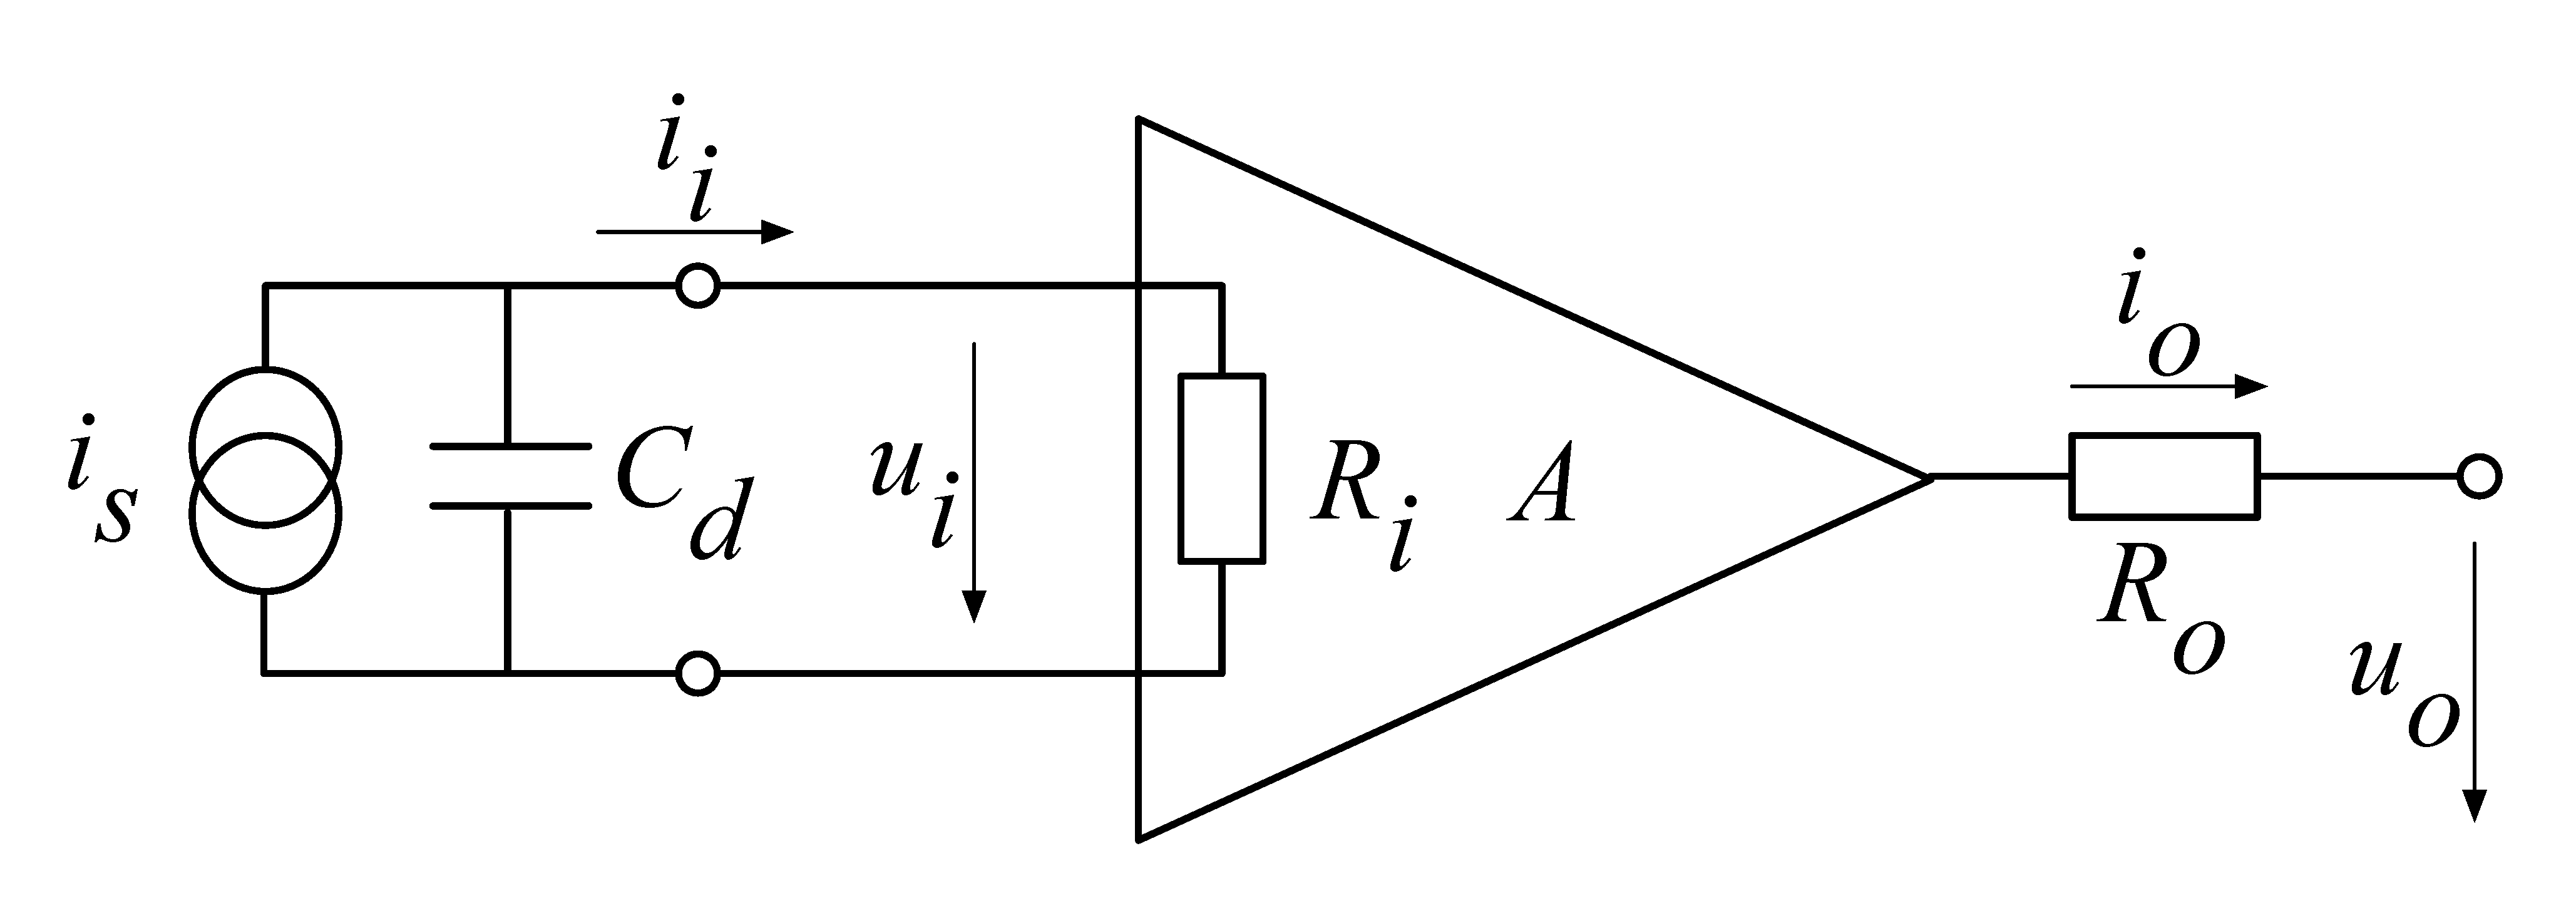
\includegraphics[width=0.50\textwidth]{02_pulse_formation/pics/plots/curramp} \label{fig:curramp}} &
\subfloat[A capacitive source and a charge amplifier.]{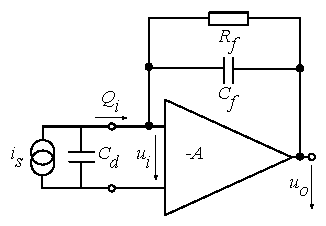
\includegraphics[width=0.40\textwidth]{02_pulse_formation/pics/plots/chgamp}  \label{fig:chgamp}}
\end{tabular}
\caption{Simplified equivalent circuits of a current and charge amplifier.}
\end{figure}


\subsubsection{Current amplifier}
Figure~\ref{fig:curramp} shows the equivalent circuit of a current source and a current amplifier. An amplifier operates in current mode if the source has a low charge collection time $t_\mathrm{c}$ with respect to the $R_\mathrm{i}C_\mathrm{d}$ time constant of the circuit. In this case the sensor capacitance discharges rapidly and the output current $i_\mathrm{o}$ is proportional to the instantaneous current $i_\mathrm{i}$. The amplifier is providing a voltage gain, so the output signal voltage $u_o$ is directly proportional to the input voltage $u_\mathrm{i}$:
\begin{equation}
u_\mathrm{o}(t) = A \cdot R_\mathrm{i} \cdot i_\mathrm{s}(t).
\end{equation}
The detector capacitance $C_\mathrm{d}$ together with the input resistance of the amplifier $R_\mathrm{i}$ defines the time constant of the signal, as shown in figure~\ref{fig:currc}. The higher $C_\mathrm{d}$, the slower is the response of the amplifier. For the case of the diamond sensor, which has the capacitance of the order of 2~pF and the input resistance of 50~$\Omega$, the resulting time constant is $\tau=10^{-10}$~s. This yields the signal rise time $t_\mathrm{r}\sim2.2\tau=2.2\times10^{-10}$~s.

\begin{figure}[!t]
\begin{center}
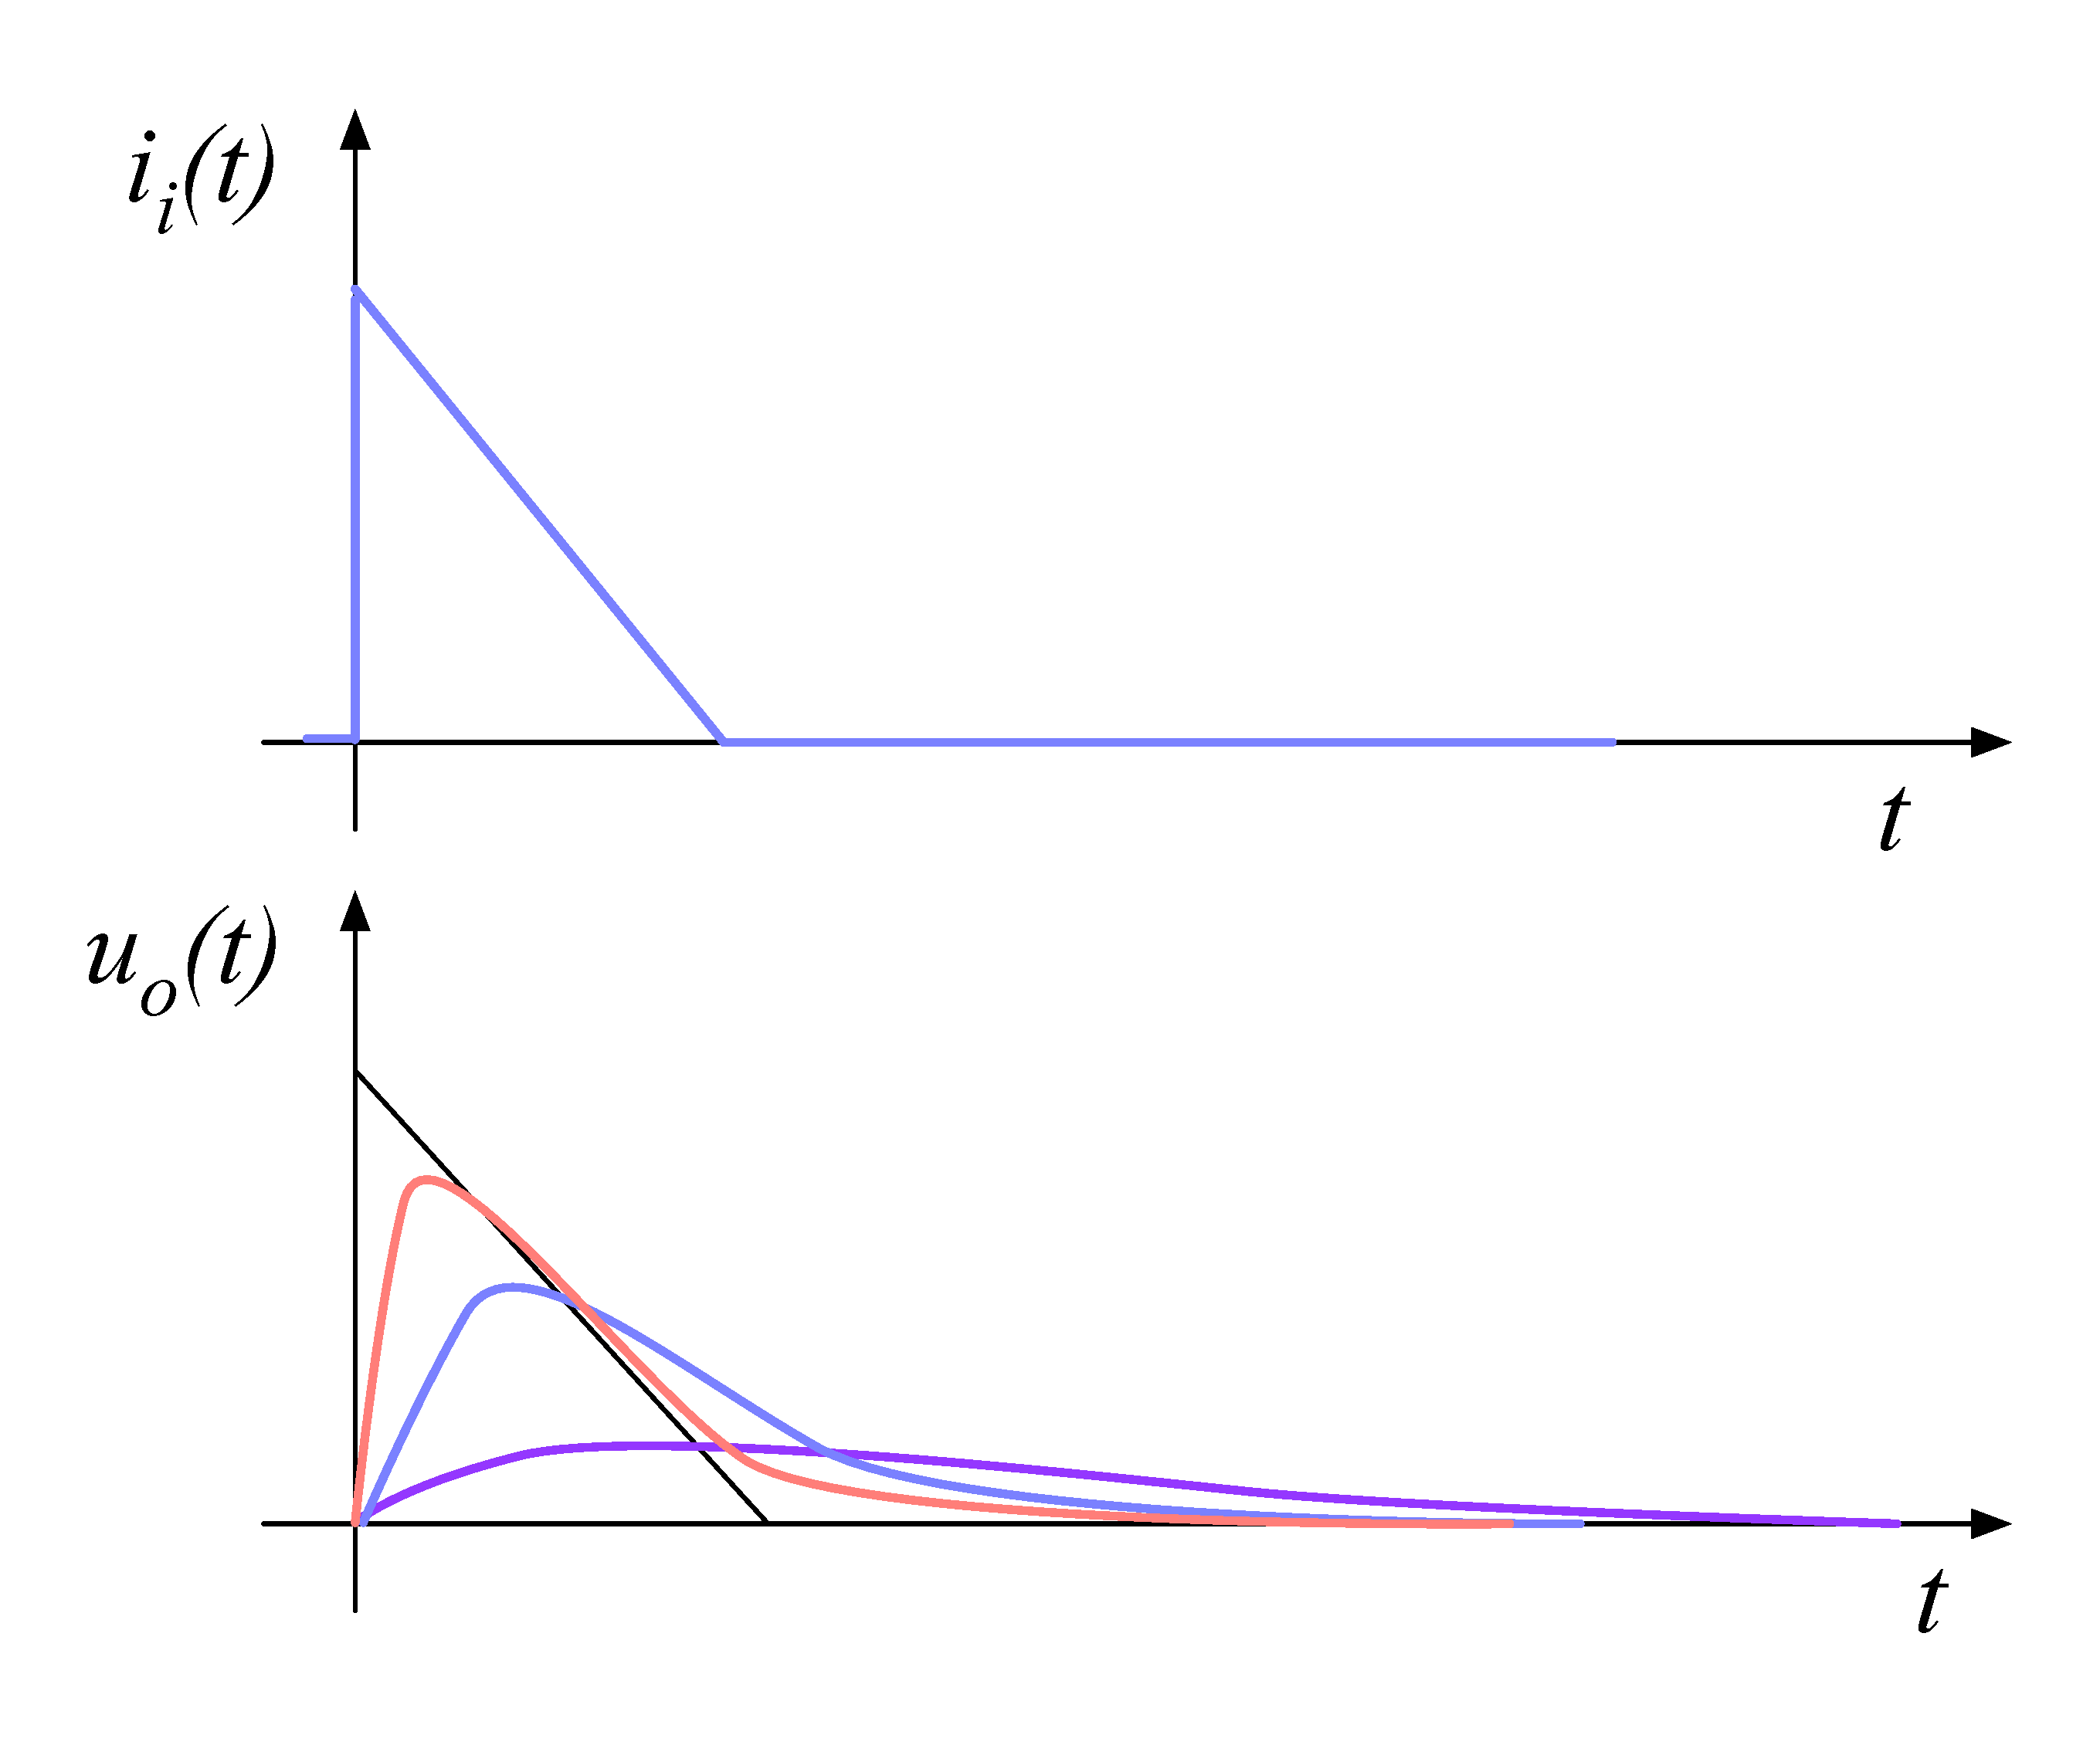
\includegraphics[width=0.7\linewidth]{02_pulse_formation/pics/plots/currrc}
\caption{Input and output signal of the current amplifier.}
\label{fig:currc}
\end{center}
\end{figure}



\subsubsection{Charge-sensitive amplifier}
%(0.5 pg)
In order to measure integrated charge in the sensor, a feedback loop is added to the amplifier, as shown in figure~\ref{fig:chgamp}. The feedback can be used to control the gain and input resistance, as well as to integrate the input signal. The charge amplifier is in principle an inverting voltage amplifier with a high input resistance. 
 
In an ideal amplifier the output voltage $u_\mathrm{o}$ equals $-Au_\mathrm{i}$. Therefore the voltage difference across the capacitor $C_\mathrm{f}$ is $u_\mathrm{f}=(A+1)u_\mathrm{i}$ and the charge deposited on the capacitor is $Q_\mathrm{f}=C_\mathrm{f}u_\mathrm{f} = C_\mathrm{f}(A+1)u_\mathrm{i}$. Since no current can flow into the amplifier, all of the signal current must charge up the feedback capacitance, so $Q_\mathrm{f} = Q_\mathrm{i}$.

In reality, however, charge-sensitive amplifiers respond much slower than is the duration of the current pulse from the sensor. In addition, a resistor is added to the feedback line in parallel to the capacitor. The resistor and capacitor define the decay time constant of the pulse, as shown in figure~\ref{fig:chgrc}. This is necessary to return the signal to its initial state to be ready for a new measurement.
\begin{figure}[!t]
\begin{center}
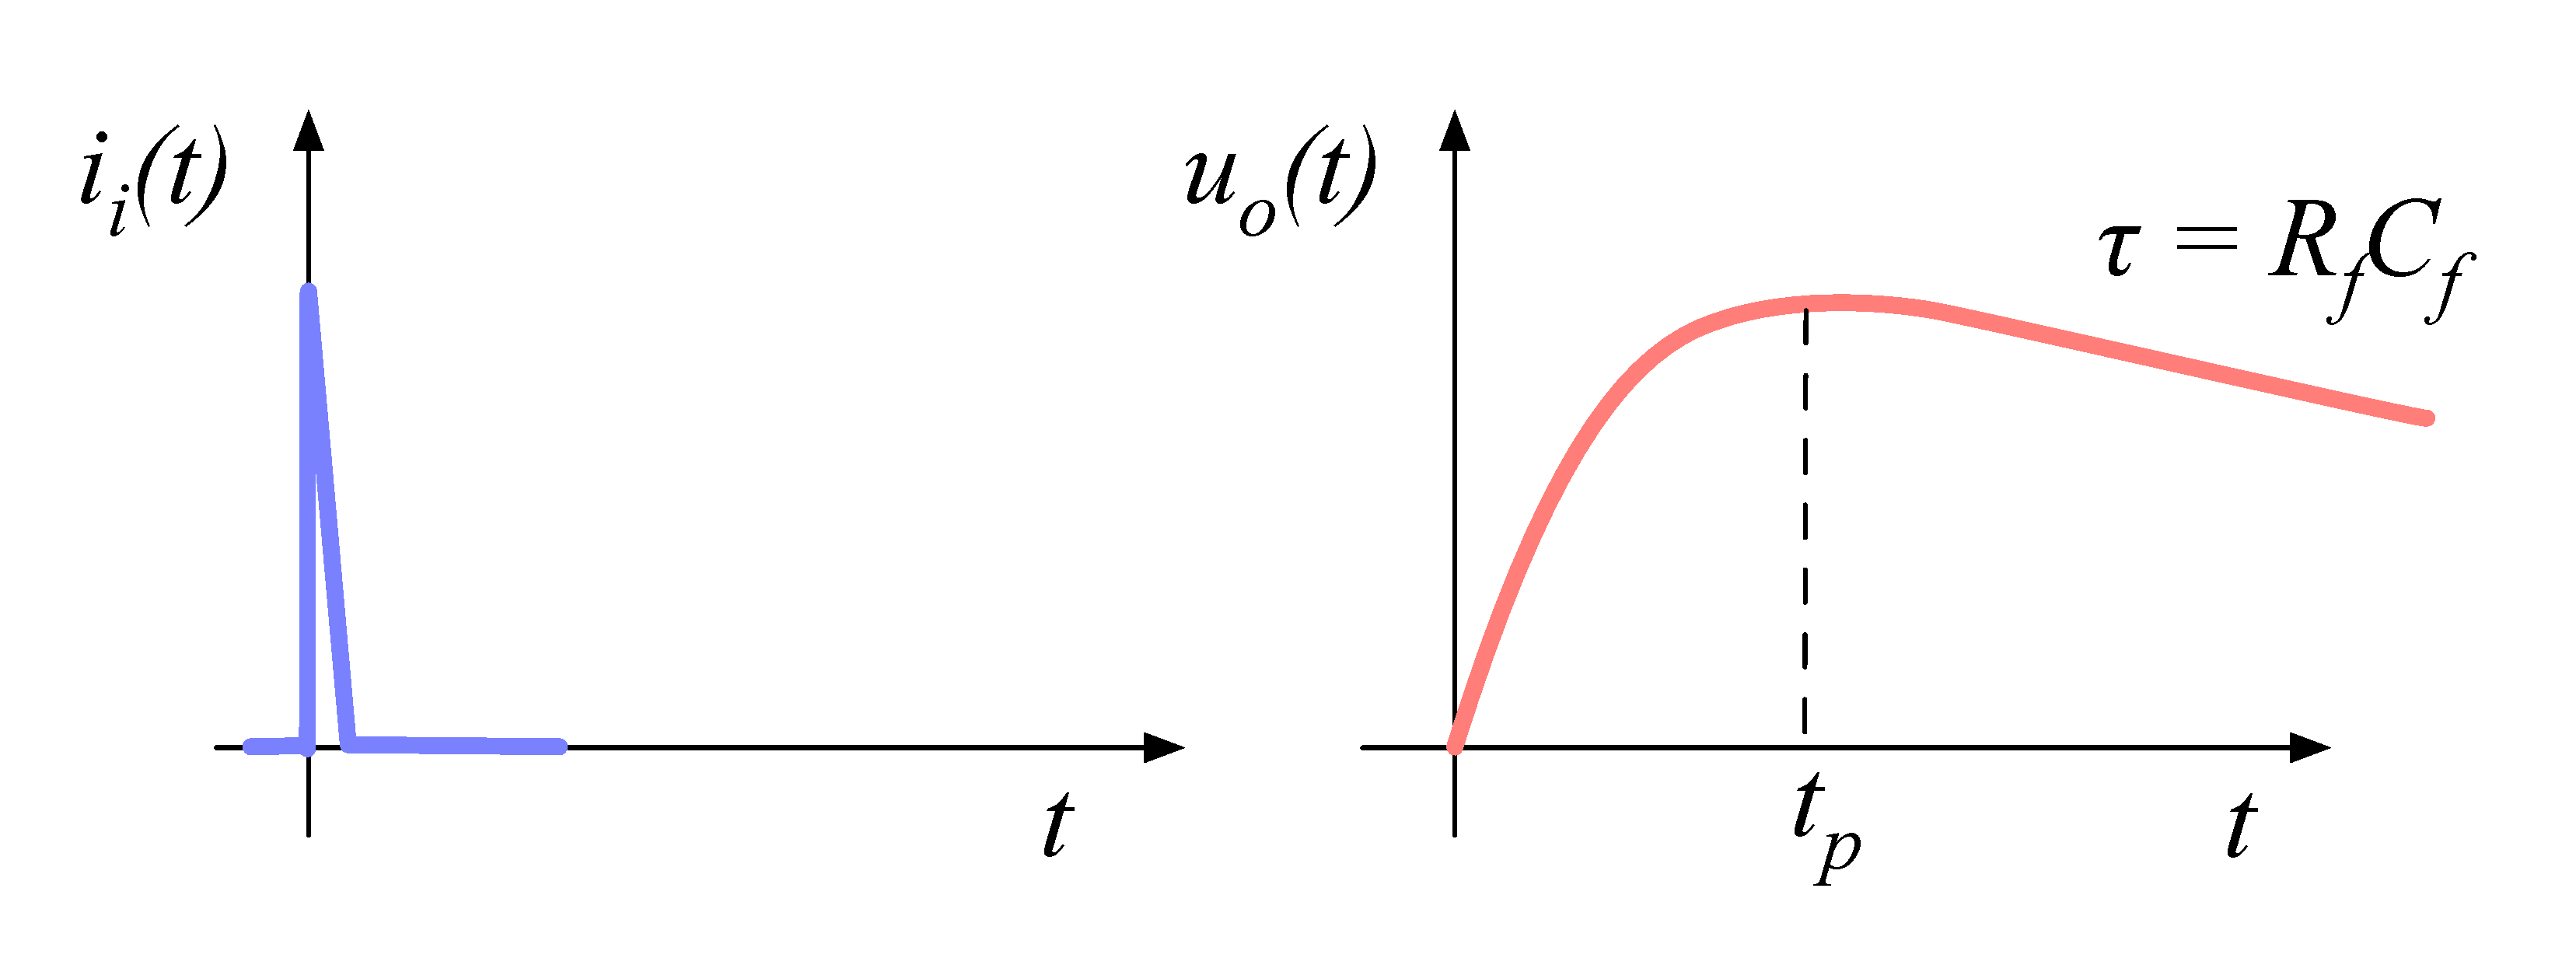
\includegraphics[width=0.7\linewidth]{02_pulse_formation/pics/plots/chgrc}
\caption{Input and output signal of the charge amplifier.}
\label{fig:chgrc}
\end{center}
\end{figure}

\subsubsection{Analogue electronic noise}
%(2 pg)
The electronic noise determines the ability of a system to distinguish different signal levels. The analogue signal contains ample information about the type and energy of incident radiation, which can quickly be erased or altered if the signal properties change. Therefore the noise contributions to the signal must be well understood to qualify the information the signal is carrying. The important contributions are listed below. Thermal or Johnson--Nyquist noise~\cite{PhysRev.32.97,PhysRev.32.110} is the dominant noise contribution in the use case for diamond detector signal amplification and therefore defines the limitations of the detector system. This noise type is generated by the random thermal motion of charge carriers. The frequency range of the thermal noise is from 0 to $\infty$ with a predominantly uniform distribution. Therefore this is nearly a white noise. The resulting signal amplitude has a Gaussian distribution. The RMS of the 
%noise amplitude
open-loop equivalent voltage is defined as
\begin{equation}
\label{eq:thermnoise}
u_\mathrm{RMS}=\sqrt{4k_BRT\Delta f}
\end{equation}
where $k_\mathrm{B}$ is the Boltzmann constant, $R$ is the input resistance of the amplifier, $T$ its temperature and $\Delta f$ the frequency range. This equation shows that it is possible to reduce the noise RMS by either (1) reducing the frequency range, (2) reducing the resistance or (3) reducing the temperature. 

Contributions of shot noise, flicker noise and burst noise and other types are not significant relative to the thermal noise. However, the contributions of external factors can severely deteriorate the signal. This means the noise produced by capacitive or inductive coupling with an external source, which causes interference in the signal. These effects can be reduced by shielding the electronics and avoiding ground loops. 

\subsection{Analogue-to-digital converters}
An analogue-to-digital converter (ADC) is a device that converts the analogue electrical signal on the input to its digital representation - a series of digital values. This involves a quantisation -- \emph{sampling} of the signal at a defined sampling period, resulting in a sequence of samples at a discrete time period and with discrete amplitude values. The resolution of the ADC is the number of output levels the ADC can quantise to and is expressed in bits. For instance, an ADC with a resolution equal to $n=8$~bit  has a dynamic range of $N=2^n=256$~steps. The resulting voltage resolution $Q_\mathrm{ADC}$ at the input voltage range of $V_\mathrm{ADC}=\pm$50~mV is then
\begin{equation}
\label{eq:mvpercnt}
Q_\mathrm{ADC}=\frac{V_\mathrm{ADC}}{2^{n}}  = \frac{100~\mathrm{mV}}{2^8~\mathrm{bit}} = 0.39~\mathrm{mV/bit}.
\end{equation} 
With a sampling period of $t_\mathrm{s}=$1~ns the sampling rate is $f_\mathrm{s}=$1~GS/s (gigasample per second).
\begin{figure}[!t]
\begin{center}
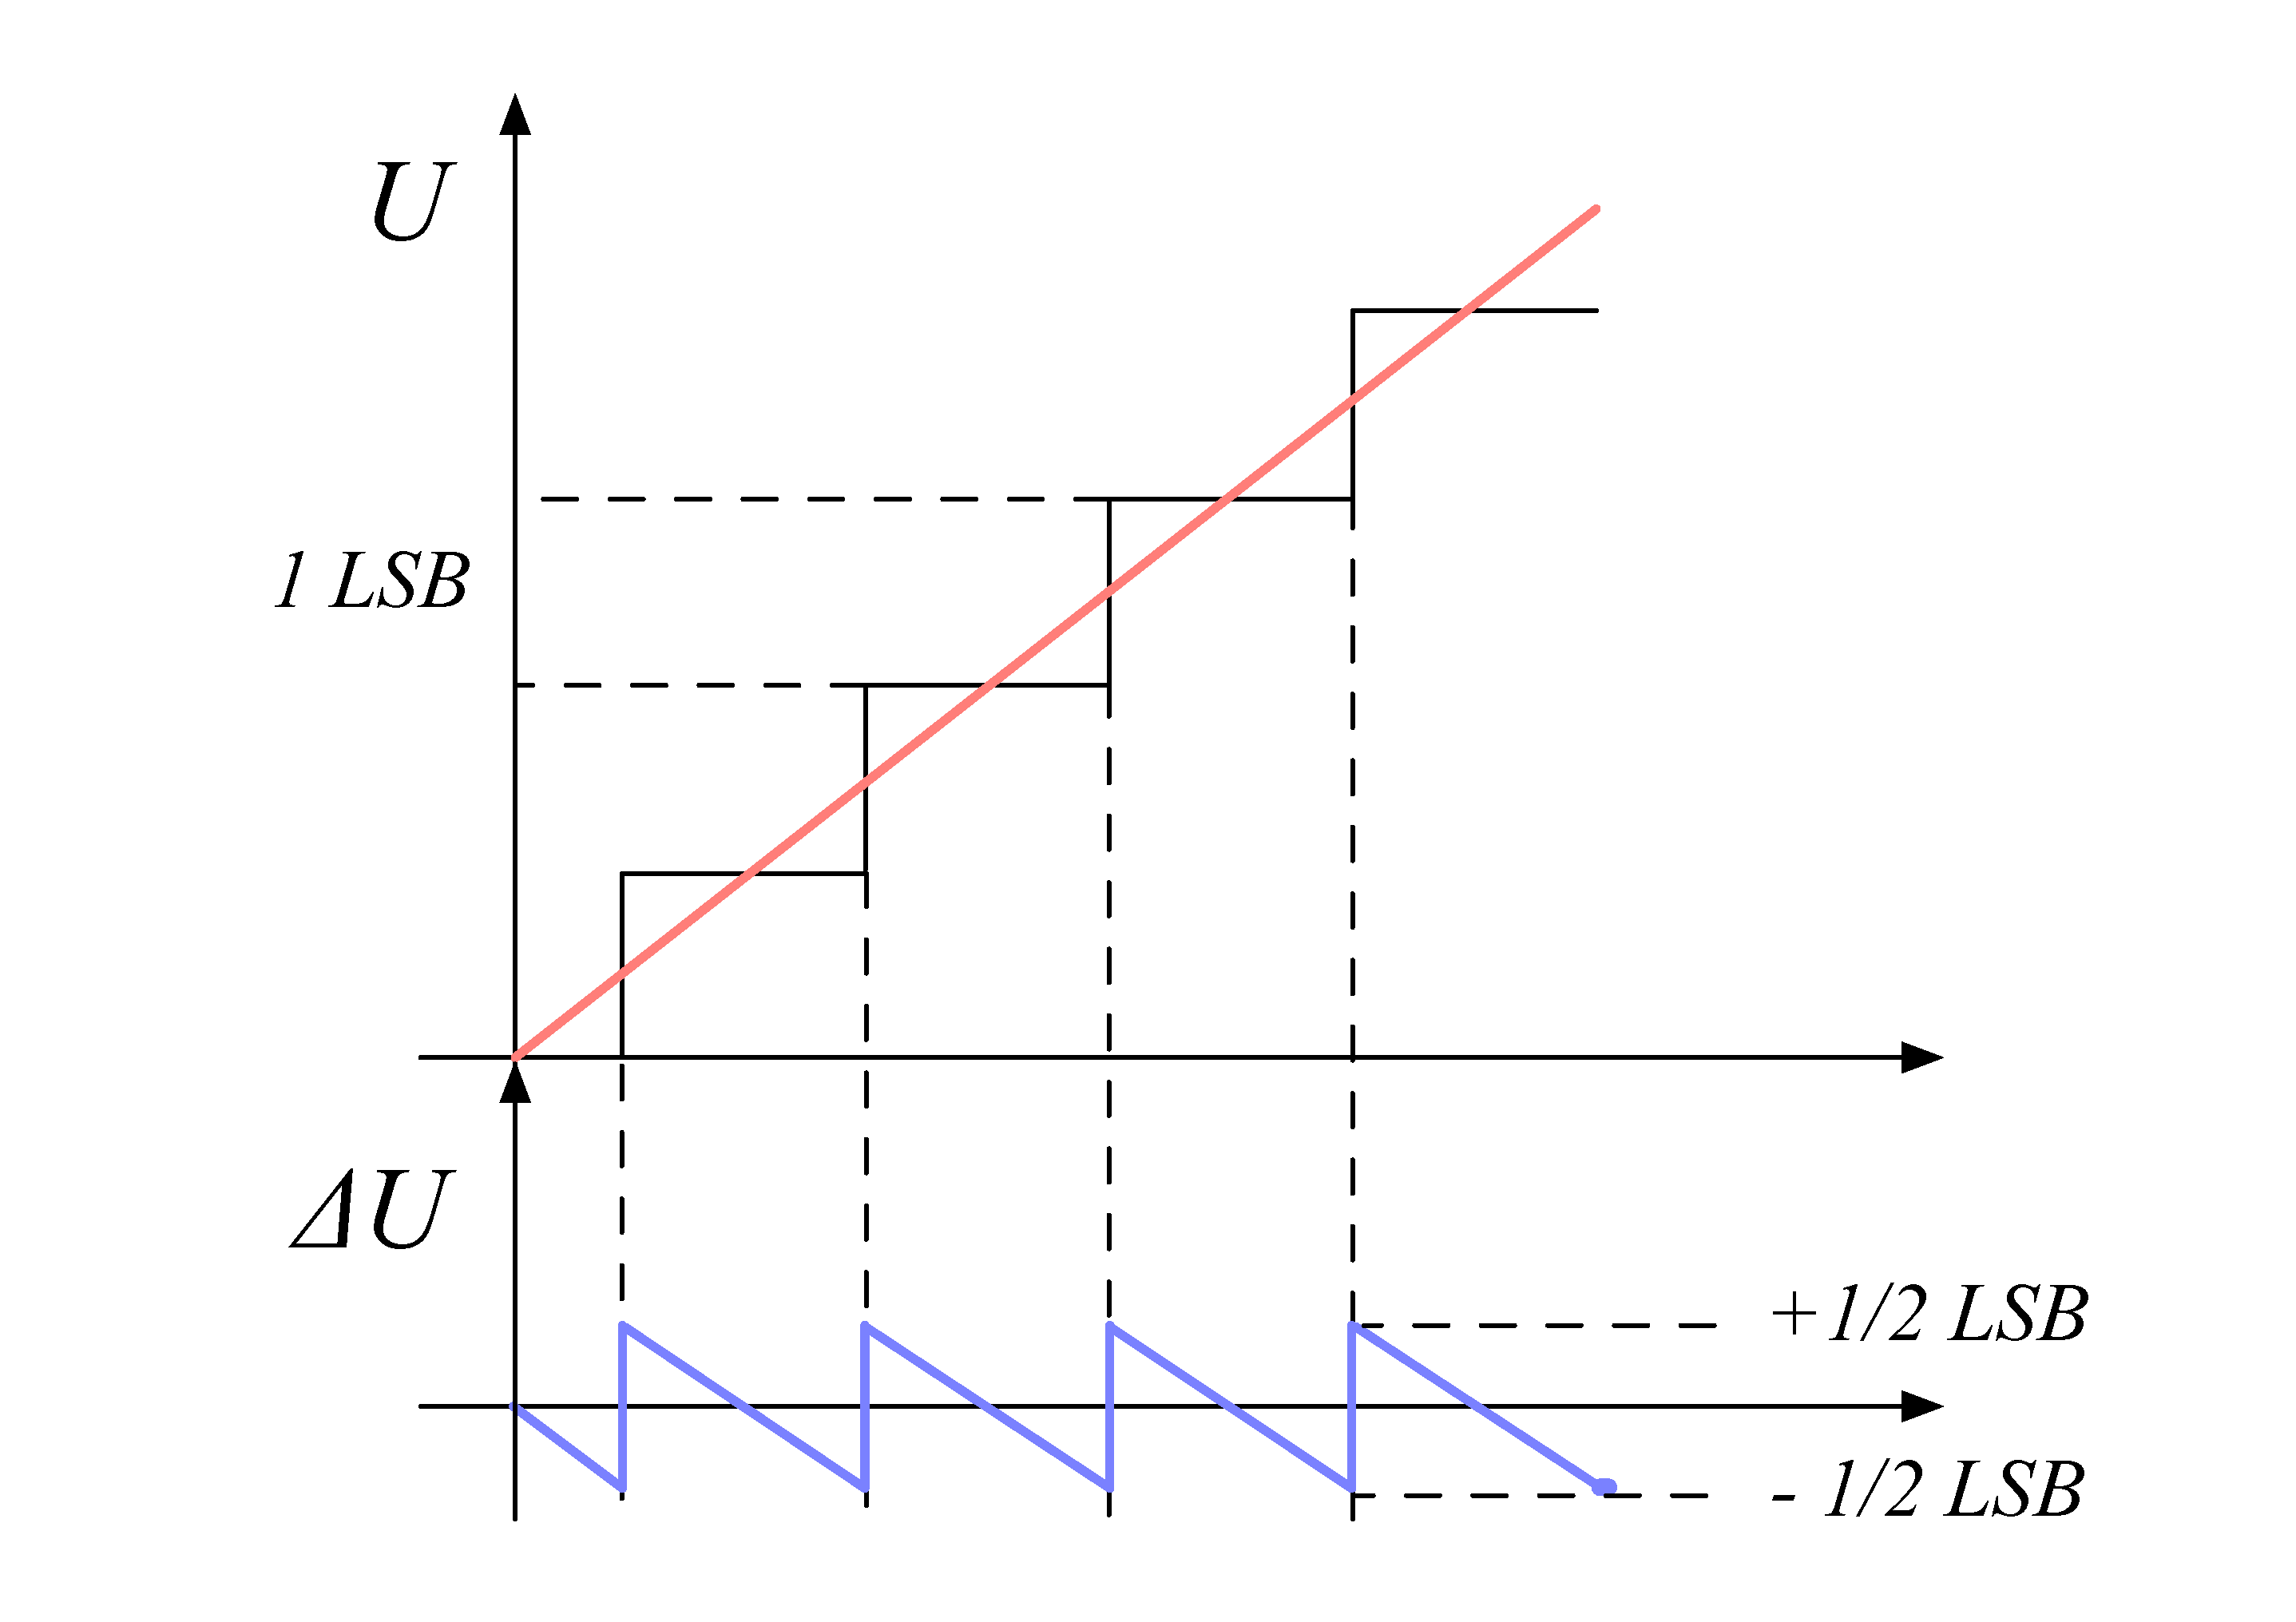
\includegraphics[width=0.7\linewidth]{02_pulse_formation/pics/plots/qerr}
\caption{Input signal digitisation and quantisation error.}
\label{fig:qerr}
\end{center}
\end{figure}

\begin{description}
\item[Quantisation error and quantisation noise] (or a round-off error) is a contribution to the overall measurement error due to digitisation (rounding). The quantisation error is defined as a difference between the actual analog value and the closest digitised representation of this value, therefore by the least significant bit (LSB), as seen in figure~\ref{fig:qerr}. The input signal amplitude is typically much larger than than the voltage resolution. In this case the quantisation error is not directly correlated with the signal and has an approximately uniform distribution. The probability density function $P(x)$ therefore has a rectangular shape bounded by ($-\frac{1}{2}$LSB, $\frac{1}{2}$LSB): 
  \begin{numcases}{P(x)=}
  \frac{1}{\mathrm{LSB}}, & $-\frac{1}{2}\mathrm{LSB}<= x <=-\frac{1}{2} \mathrm{LSB}$  \\
  0, & otherwise.
  \end{numcases}
The height equal to $\frac{1}{\mathrm{LSB}}$ preserves the integrated probability of 1. The variance of the distribution is
\begin{equation}
\label{eq:intprob}
\sigma^2 = \int P(x) (x-\mu)^2 \mathrm{d}x.
\end{equation} 
The population mean is $\mu=0$, therefore
\begin{equation}
\label{eq:intprob2}
\sigma^2 = \int_{-\frac{1}{2}\mathrm{LSB}}^{\frac{1}{2}\mathrm{LSB}} \frac{1}{\mathrm{LSB}} x^2 \mathrm{d}x 
= \frac{x^3}{3\mathrm{LSB}} \Bigg|_{ -\frac{1}{2}\mathrm{LSB} }^{\frac{1}{2}\mathrm{LSB} }
= \frac{\mathrm{LSB}^2}{12}.
\end{equation} 
The RMS of the quantisation noise is defined as the square root of the variance: 
\begin{equation}
\label{eq:qerr}
\Delta Q_\mathrm{ADC}=\sqrt{\sigma^2} =  \frac{1}{\sqrt{12}}\mathrm{LSB}\sim0.289~\mathrm{LSB}.
\end{equation} 
For the example above the quantisation error equals $\Delta Q_\mathrm{ADC}=0.11$~mV. The error depends strongly on the linearity of the ADC, but this is out of scope of this document as the devices used have ADCs with a very good linearity.
\end{description}

\subsection{Digital signal processing}
The digitised signal can be processed to extract useful information. Therefore after the signal amplification and digitisation the signal is routed in a device which handles the digital analysis. The signal can either be processed immediately (in real time) or it can be saved to a data storage for analysis at a later stage (offline). The devices carrying out the processing can be multipurpose (e.g. Field Programmable Gate Arrays) or dedicated (e.g. Application-Specific Integrated Circuits).

\begin{description}
\item[Field Programmable Gate Array] (FPGA) is an integrated circuit designed to be reprogrammable and reconfigured after manufacturing. It consists of a set of logic gates that can be interconnected in numerous combinations to carry out a set of logic operations. Many such logic operations can take place in parallel, making the FPGA a powerful tool for signal processing. FPGAs are often used during system development or in systems in which the requirements might change with time. They can be reprogrammed in the order of seconds. In addition, the logic design only needs minor changes when migrating to a newer version of the FPGA chip of the same vendor. The FPGAs also offer faster time-to-market with comparison to application-specific solutions, which have to be developed. On the other hand, the price per part can be significantly higher than for the application-specific solutions. Also, their other major disadvantages are a high power consumption and a relatively low speed as compared to more application-specific solutions. However, today's solutions are capable of clock speeds higher than 500~MHz. Together with the integrated digital signal processing blocks, embedded processors and other modules, they are already very powerful and versatile. All in all, FPGAs are a good choice for prototyping and limited production, for projects with limited requirements for speed and complexity.

\item[Application-Specific Integrated Circuit] (ASIC) is an integrated circuit designed for a specific use. The design cannot be modified after chip production, as is the case with FPGAs. On the other hand, the ASICs can be optimised to perform a required operation at a high speed and at a low power consumption. In addition, due to the specific design the size of the chip can be much smaller. ASICs can be designed as hybrid chips, containing both a digital and an analog part. Finally, ASICs can be designed to withstand much higher irradiation doses than FPGAs and can therefore be used in harsh environments like in space or in particle colliders.

To update the chip, the design has to be submitted to a foundry, which produces the new chips with a turnover time of 4---6 weeks. The costs of a submission are high, but the price per part can be reduced significantly with a high volume. To sum up, ASICs are used for high volume designs with well defined requirements where some stringent constraints in terms of power consumption and speed have to be met.
\end{description} 

\begin{figure}[!t]
%\centering
\begin{tabular}{cccc}
\subfloat{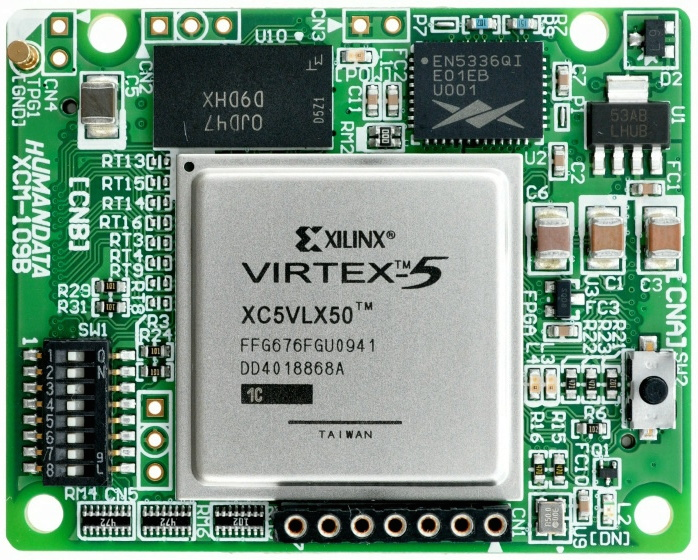
\includegraphics[width=0.47\textwidth]{02_pulse_formation/pics/fpga} \label{fig:fpga}} & 
\subfloat{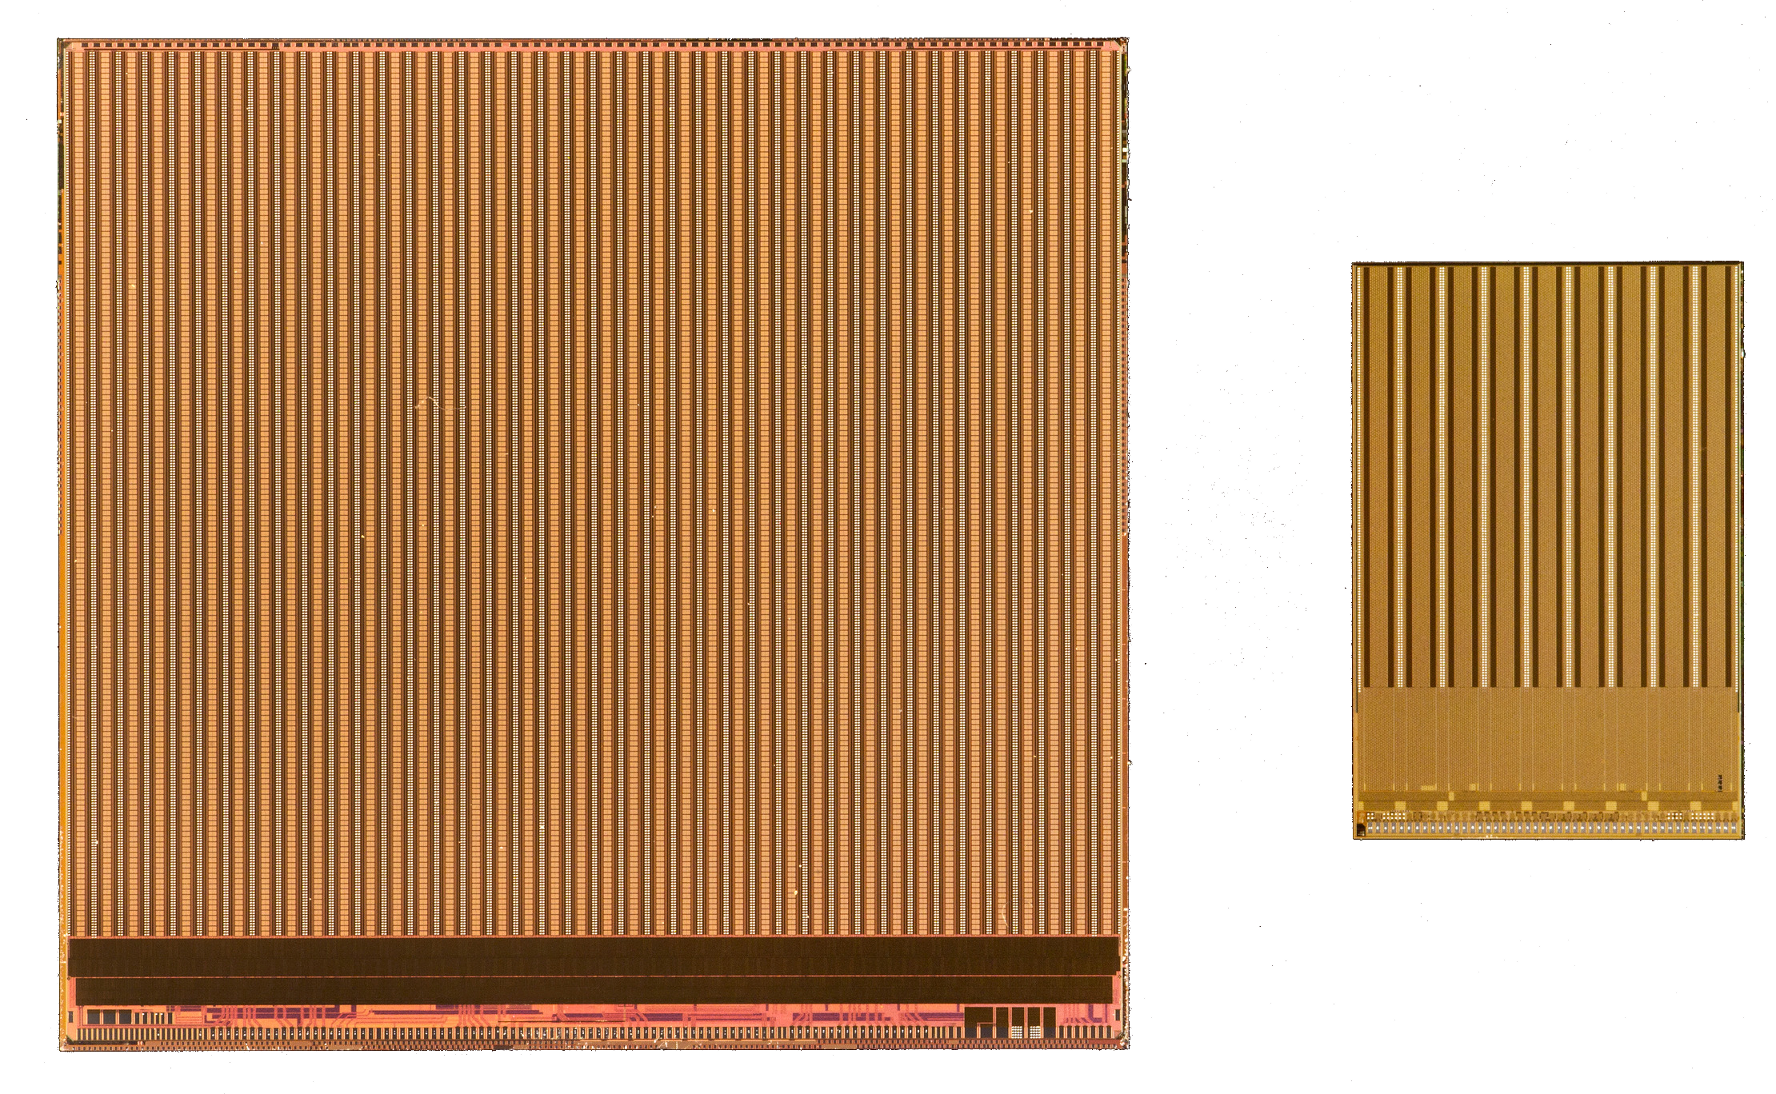
\includegraphics[width=0.47\textwidth]{02_pulse_formation/pics/asic2}  \label{fig:asic}}
\end{tabular}
\caption{An example of a Xilinx Virtex 5 FPGA~\cite{FPGA:00000} and an FE-I4 and FE-I3 ASIC chip~\cite{ASIC:00000}.}
\end{figure}
